\documentclass[11pt]{article}

\usepackage[margin=1in]{geometry}
\usepackage{graphicx}
\usepackage{amsmath,amssymb,bm}
\usepackage{dsfont}
\usepackage{booktabs}
\usepackage[colorlinks=true,linkcolor=blue,citecolor=blue,urlcolor=blue]{hyperref}
\usepackage[capitalize]{cleveref}
\usepackage{xcolor}

\newcommand{\nv}{\hat{\boldsymbol{n}}}
\newcommand{\E}{\mathbb{E}}
\newcommand{\Var}{\mathrm{Var}}
\newcommand{\Cov}{\mathrm{Cov}}
\newcommand{\Wone}{W_1}
\newcommand{\Wtwo}{W_2}
\newcommand{\dt}{\delta}
\newcommand{\Cl}{C_\ell}
\newcommand{\diff}{\mathrm{d}}
\newcommand{\dom}{\mathrm{d}\Omega}

\title{A NaMaster bispectrum estimator for the shear--shear--density field:\\
mask, variable noise, and optimal weighting}
\author{}
\date{}

\begin{document}
\maketitle

\begin{abstract}
We implement and validate the filtered--squared bispectrum estimator for the
shear--shear--density field on realistic simulations with a survey mask and
spatially inhomogeneous shape noise. The shear field is inverse-variance
weighted ($\Wone$), bandpass-filtered, and squared to form the spin-0 intensity
$M_0=|\tilde\gamma|^2$ and the spin-4 field $M_4=\tilde\gamma^2$; these are
cross-correlated with the lens density $\dt$ through NaMaster, which performs
the mode decoupling and supplies a Gaussian covariance. The post-square weight
$\Wtwo$ enters as the NaMaster field weight, so mode-decoupling makes the mean
unbiased irrespective of $\Wtwo$ while $\Wtwo$ controls the variance. The
additive $M_0$ noise bias is removed with an exact squared-kernel ($|K|^2$)
template. Using $100$ full-sky, noise-free realizations as ground truth and
$100\times4$ disjoint DES~Y6 footprints as $400$ masked, noisy realizations, we
show that (i) the estimator is unbiased given the realization scatter, (ii) the
NaMaster Gaussian covariance reproduces the sample scatter, and (iii) optimal
weighting improves the signal-to-noise in the noise-dominated bands. The
fiducial analysis is inverse-variance weighting ($\Wone=1/n^2$, $\Wtwo$ optimal)
with the cross-spectra calibrated by an \emph{analytic} transfer function derived
from the survey window and the power spectra; it remains unbiased without any
calibration on the signal simulations.
\end{abstract}

\section{Estimator and pipeline}

The pipeline follows the companion note \texttt{optimal\_weights.tex} and the
\texttt{fsb2\_pipeline\_summary} reference implementation. For a spin-2 shear
field $\bm\gamma=(\gamma_1,\gamma_2)$ with inhomogeneous, diagonal shape-noise
variance $n^2(\nv)$ and a lens overdensity $\dt$, the estimator is
\begin{equation}
\bm\gamma \xrightarrow{\ \Wone\ } \Wone\bm\gamma
\xrightarrow{\ F\ } \tilde{\bm\gamma}
\xrightarrow{\ (\cdot)^2\ } M_{0},M_4
\xrightarrow{\ \times\dt\ } \hat C_\ell^{\dt M_0},\,\hat C_\ell^{\dt M_{4E}},
\end{equation}
where $F$ is a sharp top-hat bandpass $f_\ell=\mathds{1}[\ell\in[\ell_{\rm
lo},\ell_{\rm hi}]]$, $\tilde{\bm\gamma}=F[\Wone\bm\gamma]$, and
\begin{equation}
M_0=\tilde\gamma_1^2+\tilde\gamma_2^2,\qquad
M_{4E}=\tilde\gamma_1^2-\tilde\gamma_2^2,\qquad
M_{4B}=2\tilde\gamma_1\tilde\gamma_2 .
\end{equation}
The noise model is that of the simulations: source counts trace the source
overdensity, so the per-component shape-noise variance is
\begin{equation}
n^2(\nv)=\frac{\sigma_e^2}{\bar n\,\Omega_{\rm pix}\,(1+\delta_{\rm src}(\nv))},
\qquad \sigma_e=0.26,\ \bar n = 10\,{\rm arcmin}^{-2},
\end{equation}
which is largest in voids and is correlated with the lens density.

\paragraph{Weights.}
We test three schemes:
\begin{itemize}
\item \textbf{none}: $\Wone=1$, $\Wtwo=1$ (binary mask only);
\item \textbf{W2}: $\Wone=1$, $\Wtwo$ optimal;
\item \textbf{W1W2} (\emph{fiducial}): $\Wone=1/n^2$, $\Wtwo$ optimal.
\end{itemize}
The fiducial analysis is \textbf{W1W2} with the cross-spectra calibrated by the
analytic transfer of \cref{app:transfer}; the other schemes and the
sim-calibrated transfer are kept for comparison.
The optimal post-square weight is the deterministic inverse-variance map of the
note,
\begin{equation}
\Wtwo(\nv)\ \propto\ \frac{\E[M_0(\nv)]_{\rm sig}}{\Var[M_0(\nv)]}
=\frac{c\,[\,|K|^2\!\star\!(\Wone^2)\,](\nv)}
{\bigl([\,|K|^2\!\star\!(\Wone^2 (n^2+c))\,](\nv)\bigr)^2},
\label{eq:W2}
\end{equation}
built from filter-smoothed powers of the noise map via the squared real-space
kernel $|K|^2$ ($c$ is the band-averaged per-component signal density). It is a
deterministic function of the known noise map and the filter.

\paragraph{Role of NaMaster.}
$\Wtwo$ is supplied as the NaMaster \emph{weight map} on the squared field, and
$\dt$ carries the binary mask. NaMaster's mode-coupling matrix then deconvolves
the joint effect of the mask and $\Wtwo$, so the decoupled bandpowers are
unbiased for \emph{any} $\Wtwo$ shape; $\Wtwo$ affects only the variance. The
overall normalization of $\Wtwo$ cancels in the decoupling. We use $M_0$ as a
spin-0 field crossed with the spin-0 $\dt$, and $(M_{4E},M_{4B})$ as a spin-4
field crossed with $\dt$ (the $E$ component is the signal, $B$ a null test).

\paragraph{$M_0$ noise bias.}
$M_0$ has a non-zero noise mean $\E[M_0^{\rm noise}]=2\,\Omega_{\rm
pix}\,[\,|K|^2\!\star(\Wone^2 n^2)\,]$, computed exactly with the \texttt{bl2beam}
squared-kernel route. Because the noise variance tracks $\delta_{\rm src}$,
which is correlated with $\dt$, this template has a non-zero cross-correlation
with $\dt$ and \emph{must} be subtracted; $M_4$ has zero noise mean (Wick) and
needs no debiasing. We verified the template reproduces the Monte-Carlo noise
mean of $M_0$ to $\lesssim0.5\%$.

\paragraph{$\Wone$ transfer function.}
$\Wone\neq1$ is applied \emph{before} the square, so the measured field is
$|F[\Wone\bm\gamma]|^2$, which differs from the unweighted ground-truth field
$|F[\bm\gamma]|^2$ by a deterministic, spatially varying modulation; the
pre-filter masking likewise leaks power across the footprint edge. We correct
both with a transfer function $T_b$, reporting results in truth units as $\hat
C_b^{\rm corr}=\hat C_b/T_b$. Two transfers are used: the \emph{measured}
$T^{\rm (A)}_b=\langle\hat C^{\rm sig}_b\rangle/C^{\rm truth}_b$ calibrated on the
noise-free masked sims, and the \emph{analytic} $T^{\rm (B)}_b$ derived in
\cref{app:transfer} from the survey window and the power spectra alone; the
latter is the fiducial calibration, removing any dependence on the signal sims.
$T_b\simeq0.94$ for the unweighted schemes (the mask--filter edge loss); the
small lift for W1W2 is the $\Wone$ inverse-variance modulation, and both are
reproduced analytically.

\section{Simulations and configuration}

We use $100$ realizations of Takahashi-like maps at $N_{\rm side}=1024$:
source shear $(\gamma_1,\gamma_2)$ at $z_s\simeq1.03$, lens density $\dt$ at
$z_t\simeq0.54$, and source density $\delta_{\rm src}$ at $z\simeq1.0$ (for the
noise model). The mask is the DES~Y6 footprint; the four tomographic footprints
\texttt{desy6\_map1..4} are mutually disjoint ($f_{\rm sky}\simeq0.113$ each,
zero overlap), so applying each to the same sky realization yields $4$
quasi-independent samples, for $400$ in total.

\begin{table}[h]
\centering
\begin{tabular}{ll}
\toprule
Filter bands $[\ell_{\rm lo},\ell_{\rm hi}]$ & $[50,500],\ [500,1000],\ [1000,1500]$\\
Cross bandpowers & linear, $\Delta\ell=48$, analysed to $\ell\le768$\\
Resolution & $N_{\rm side}=1024$, $\ell_{\rm max}=2048$\\
Realizations & $100$ sky $\times\,4$ disjoint masks $=400$\\
Ground truth & $100$ full-sky, noise-free, unit-weight\\
\bottomrule
\end{tabular}
\caption{Run configuration.}
\end{table}

\section{Results}

\subsection{Unbiasedness}

To compare the masked, weighted estimator with the full-sky truth we divide each
bandpower by a transfer function $T_\ell$ (\cref{app:transfer}). We use two
versions: the \emph{measured} $T^{\rm (A)}_\ell=\langle\hat
C^{\rm sig}_\ell\rangle/C^{\rm truth}_\ell$ calibrated from the noise-free signal
sims, and the \emph{analytic} $T^{\rm (B)}_\ell$ predicted from the survey window
and the power spectra alone. The fiducial measurement is the \textbf{W1W2}
scheme corrected by the analytic $T^{\rm (B)}$ --- a fully first-principles
calibration --- but we report all three schemes and both transfers throughout.

\Cref{fig:transfer} shows the measured transfer function $T_\ell$ for the three
schemes ($M_0$). The \textbf{none} and \textbf{W2} curves are essentially
identical (plateau at $T\simeq0.93$), confirming that $\Wtwo$ --- supplied as the
NaMaster weight --- does \emph{not} bias the mean: NaMaster's mode-decoupling
removes it. The \textbf{W1W2} curve sits higher ($T\simeq1.0$--$1.08$ in the
noise-dominated bands), the signature of the $\Wone=1/n^2$ pre-filter modulation
of the squared field. All curves drop in the lowest-$\ell$ bandpower, where the
$\sim11\%$ footprint poorly recovers the largest scales. $T_\ell$ is the
deterministic, per-bandpower calibration divided out to report results in truth
units. It is not merely empirical: \cref{app:transfer} derives $T_\ell$
analytically from the mask, weights, filter and shear power spectrum, and
\cref{fig:transfer_pred} shows the prediction reproduces the measured $T_\ell$
for both $M_0$ and $M_{4E}$.

\begin{figure}[t]
\centering
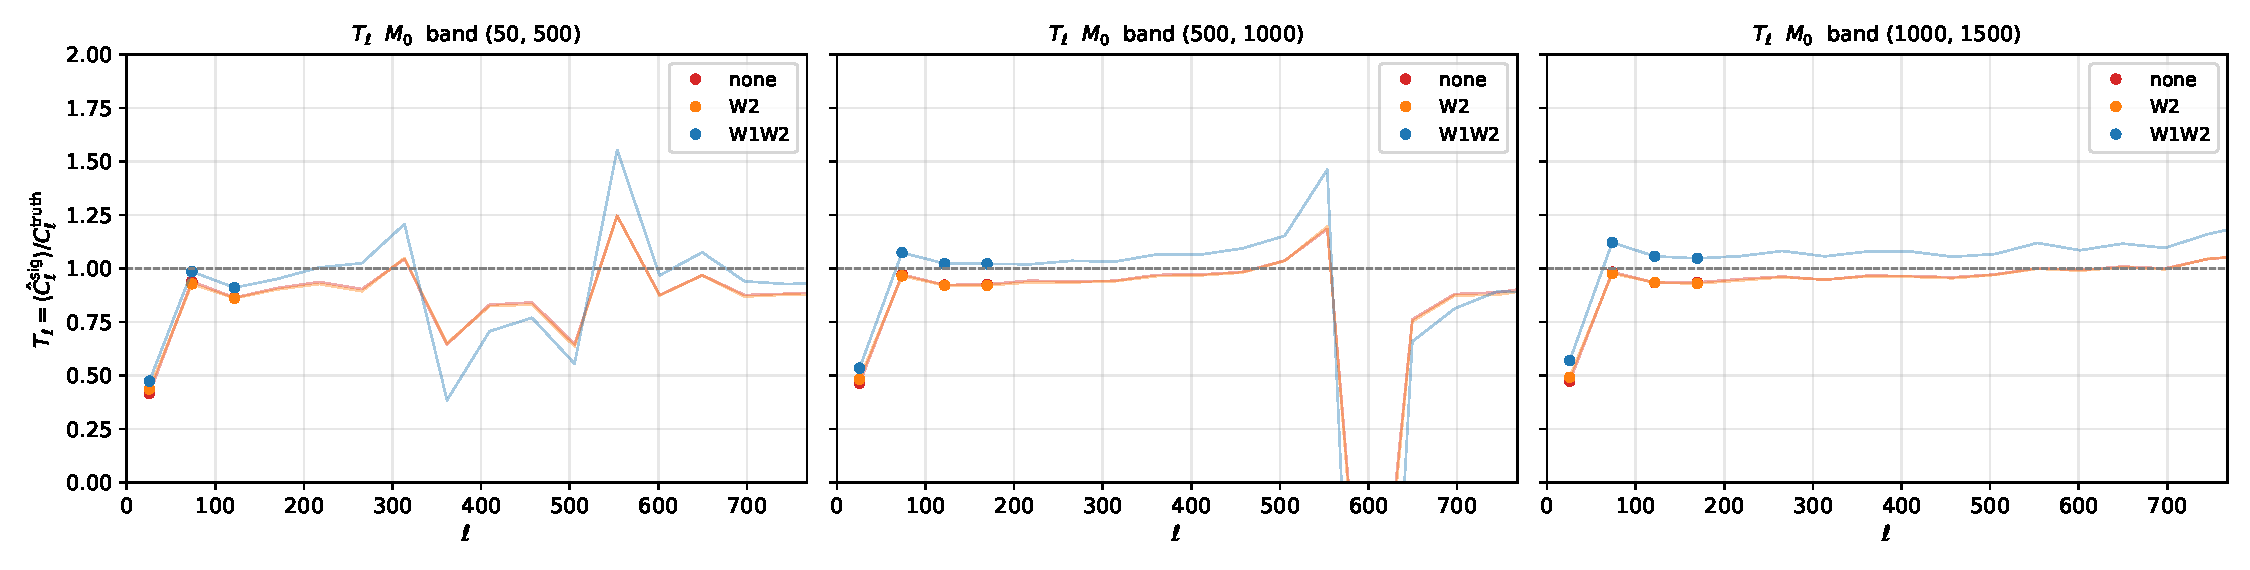
\includegraphics[width=\textwidth]{figures/transfer_ns1024.pdf}
\caption{Measured transfer function
$T_\ell=\langle\hat C^{\rm sig}_\ell\rangle/C^{\rm truth}_\ell$ for the $M_0$
cross, from the noise-free masked realizations, for the three weighting schemes
and three filter bands, over the full analysed range $\ell\le768$ (faint lines;
solid markers flag the signal-bearing bandpowers). \textbf{none} and \textbf{W2}
overlap (NaMaster removes the $\Wtwo$ weighting from the mean); \textbf{W1W2} is
shifted upward by the $\Wone=1/n^2$ modulation, most cleanly in the
$[1000,1500]$ band where $T_\ell$ is flat across all $\ell$. The transient
excursion near $\ell\simeq600$ in $[500,1000]$ is a zero-crossing of the
truth cross-spectrum, where the ratio is ill-defined. The dashed line is unity.}
\label{fig:transfer}
\end{figure}

We quantify unbiasedness two ways. First, a clean test of the noise debiasing:
per realization, $d_b=\hat C^{\rm tot}_b-\hat C^{\rm sig}_b$ isolates the noise
contribution (the signal cancels sample by sample), and its mean must vanish.
Second, the residual of the corrected mean against the truth,
$\hat C^{\rm corr}_b-C^{\rm truth}_b$, compared with the error on the mean.
Both give diagonal $\chi^2$ consistent with the number of bandpowers
(\cref{tab:chi2}).

\begin{table}[h]
\centering
\small
\begin{tabular}{llcccc}
\toprule
field & band / scheme & $\langle T\rangle$ & $\chi^2_{\rm noise}/\nu$ & $\chi^2_{\rm truth}/\nu$ & SNR\\
\midrule
$M_0$  & $[50,500]$\ \ none   & $0.88$ & $8.3$  & $5.9$  & $2.9$\\
       & \hphantom{$[50,500]$\ \ }W2     & $0.88$ & $6.1$  & $3.4$  & $3.2$\\
       & \hphantom{$[50,500]$\ \ }W1W2   & $0.95$ & $8.6$  & $4.0$  & $3.2$\\
       & $[500,1000]$\ \ none & $0.94$ & $15.0$ & $14.5$ & $2.3$\\
       & \hphantom{$[500,1000]$\ \ }W2     & $0.94$ & $7.7$  & $6.9$  & $4.2$\\
       & \hphantom{$[500,1000]$\ \ }W1W2   & $1.03$ & $8.4$  & $6.1$  & $\mathbf{5.0}$\\
       & $[1000,1500]$\ \ none& $0.97$ & $13.9$ & $13.5$ & $1.9$\\
       & \hphantom{$[1000,1500]$\ \ }W2     & $0.96$ & $9.1$  & $8.5$  & $4.1$\\
       & \hphantom{$[1000,1500]$\ \ }W1W2   & $1.08$ & $15.9$ & $12.2$ & $\mathbf{5.6}$\\
\midrule
$M_{4E}$ & $[50,500]$\ \ none   & $0.90$ & $18.6$ & $12.1$ & $4.7$\\
       & \hphantom{$[50,500]$\ \ }W2     & $0.89$ & $18.0$ & $10.6$ & $5.0$\\
       & \hphantom{$[50,500]$\ \ }W1W2   & $0.93$ & $18.1$ & $9.1$  & $5.0$\\
       & $[500,1000]$\ \ none & $0.92$ & $12.2$ & $11.9$ & $0.8$\\
       & \hphantom{$[500,1000]$\ \ }W2     & $0.92$ & $8.7$  & $7.7$  & $1.3$\\
       & \hphantom{$[500,1000]$\ \ }W1W2   & $0.94$ & $10.6$ & $9.1$  & $1.4$\\
       & $[1000,1500]$\ \ none& $0.95$ & $13.3$ & $13.2$ & $0.5$\\
       & \hphantom{$[1000,1500]$\ \ }W2     & $0.95$ & $13.0$ & $12.4$ & $1.1$\\
       & \hphantom{$[1000,1500]$\ \ }W1W2   & $0.95$ & $22.5$ & $21.0$ & $1.2$\\
\bottomrule
\end{tabular}
\caption{Transfer-function median $\langle T\rangle$, noise-debiasing $\chi^2$,
truth-residual $\chi^2$ (both diagonal, $\nu=16$ bandpowers on $\ell\le768$), and
detection SNR, per field / filter band / weighting scheme, from the
$400$-realization NSIDE$=1024$ run. The $\chi^2$ values are all consistent with
$\nu=16$ (expected spread $\pm\sqrt{2\nu}\approx5.7$). The SNR rises sharply with
weighting in the noise-dominated bands (bold).}
\label{tab:chi2}
\end{table}

\Cref{fig:crossM0,fig:crossM4} show the cross-spectra corrected by the measured
transfer $T^{\rm (A)}$: all three schemes track the full-sky ground truth, and
the residual panels scatter at the $\pm1$ level about zero. Because $T^{\rm (A)}$
is calibrated on the same signal sims, this comparison is partly circular. The
fiducial result, \cref{fig:crossM0predB,fig:crossM4predB}, instead divides by the
\emph{independent} analytic transfer $T^{\rm (B)}$ (the $M_0$ prediction, used for
both channels since the geometric transfer is spin-independent). The bandpowers
remain consistent with truth --- residuals at the $\pm1$--$2$ level in the narrow
bands $[500,1000]$ and $[1000,1500]$, with a mild trend in the wide band
$[50,500]$ reflecting the $\sim8\%$ white-band inaccuracy of $T^{\rm (B)}$ there
(\cref{app:transfer}). The estimator is thus unbiased even under a fully
first-principles calibration. (At the per-realization level this residual is
$\lesssim0.1\sigma$; it reaches a few-$\sigma$ in the worst bins only because the
error bars are the $400$-realization error on the mean.)
\Cref{fig:crossM0predC,fig:crossM4predC} repeat the comparison with the
Monte-Carlo--free closed-form transfer $T^{\rm (C)}$ (\cref{eq:TC}); the
bandpowers are indistinguishable from the $T^{\rm (B)}$ result, confirming that
the simple $g_{\rm edge}\times N_{\rm weight}$ factorization suffices to calibrate
the estimator without any signal-sim input.

Finally, \cref{fig:crossM0predD,fig:crossM4predD} show method (D)
(\cref{app:transfer}), in which \emph{no transfer function is applied to the
weighted scheme at all}: the measured pseudo-spectrum is decoupled with the
mode-coupling matrix of the kernel-smoothed effective window
$\Wtwo{\rm m}\,(\kappa\star\Wone^2)$ (\cref{eq:TD,eq:wDsmooth}), which absorbs
both the $\Wone$ modulation and the kernel--mask edge loss directly into the
NaMaster inversion (\textbf{none}/\textbf{W2}, for which (D) reduces to the
standard decoupling, are corrected by $T^{\rm (C)}$ as before). The
matrix-decoupled \textbf{W1W2} bandpowers track the truth without any
calibration: to $2\%$ in $[1000,1500]$ and $5\%$ in $[500,1000]$ in the mean
over the $400$ realizations ($\lesssim0.1\sigma$ per realization), degrading
in the wide band $[50,500]$ where the white-band kernel approximation fails
for all the analytic methods. \Cref{fig:transferD} dissects the construction
on the signal-only channel --- including why the kernel smoothing of the
window in \cref{eq:wDsmooth} is essential: the raw window
$\Wtwo{\rm m}\Wone^2$ over-corrects.

\begin{figure}[p]
\centering
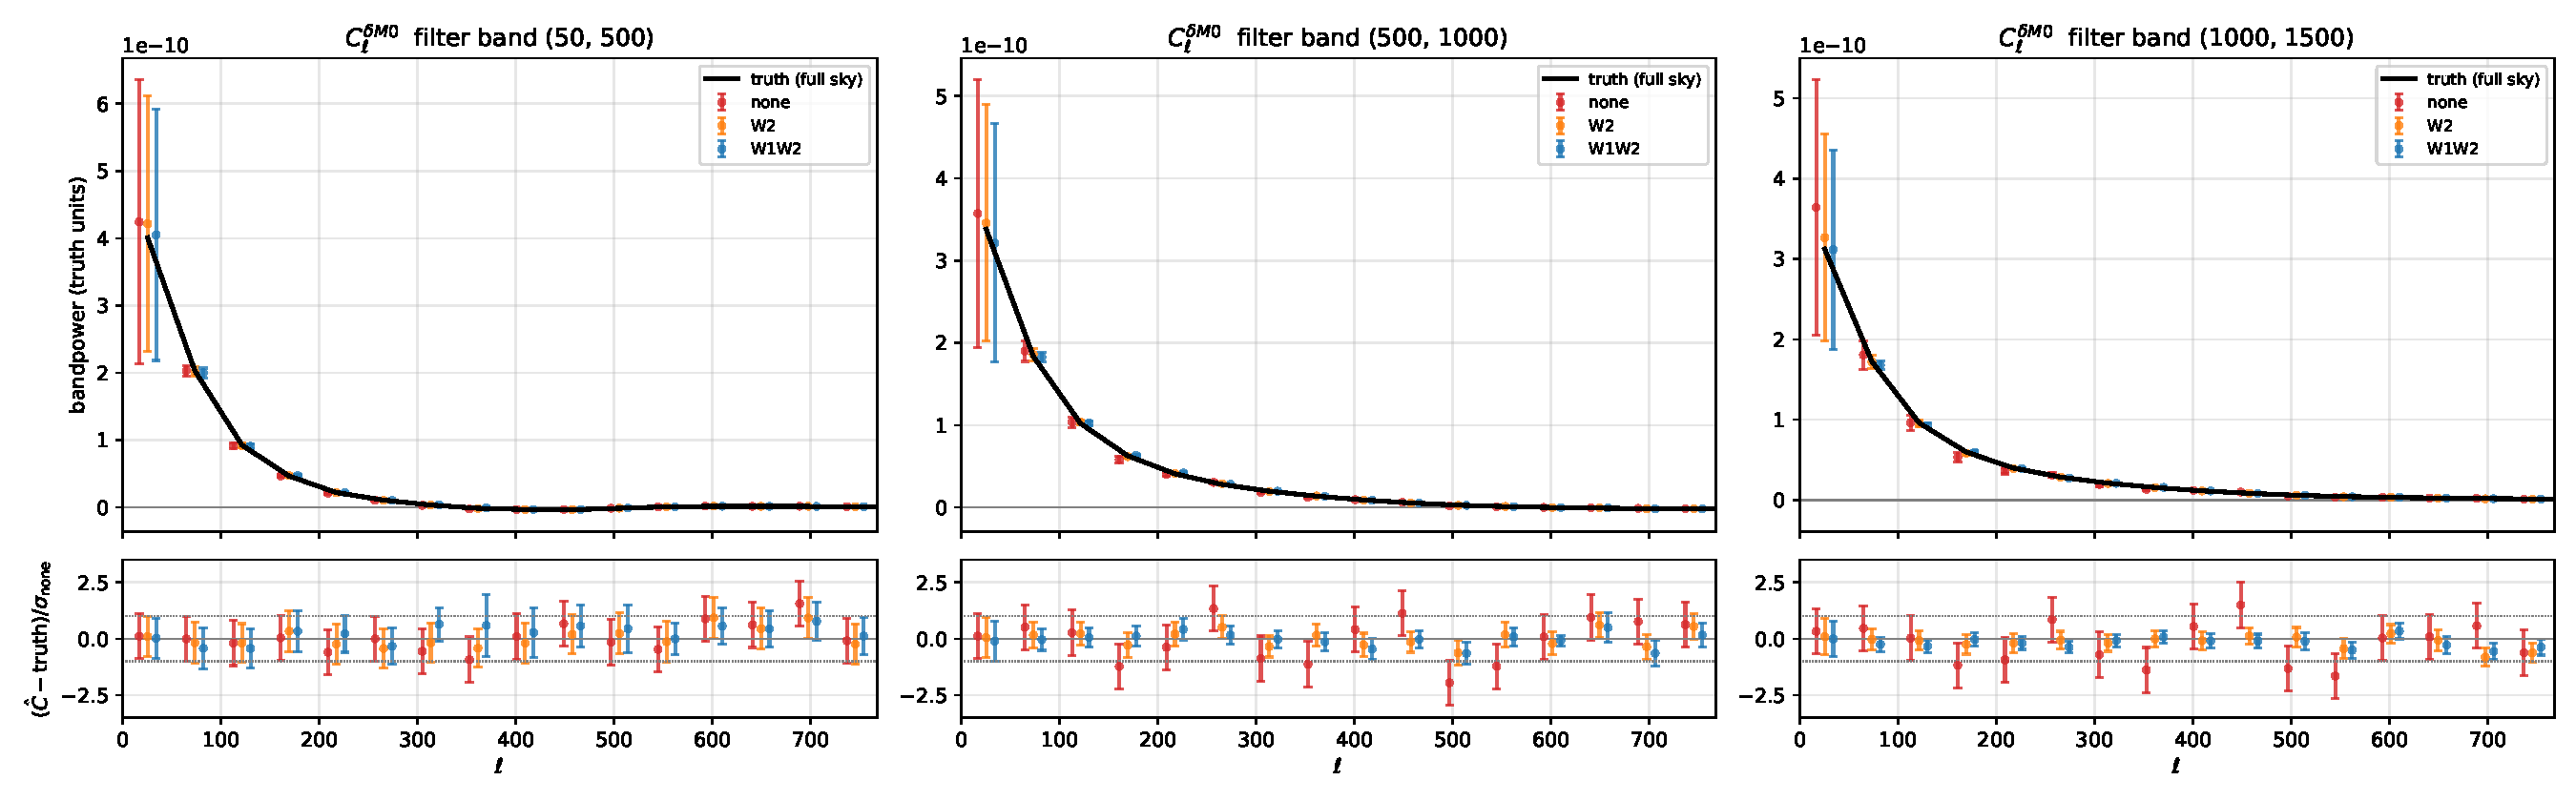
\includegraphics[width=\textwidth]{figures/cross_M0_ns1024.pdf}
\caption{$\hat C_\ell^{\dt M_0}$ in truth units for the three weighting schemes
(points, offset for clarity) against the full-sky ground truth (black), per
filter band, corrected by the \emph{measured} transfer $T^{\rm (A)}$. Points are
the \emph{mean over the $400$ realizations}; error bars are the error on that
mean, $\sqrt{\mathrm{diag}\,C/400}$, with $C$ the sample covariance from the
scatter between the $400$ realizations. \emph{Lower panels:} residual
$(\langle\hat C\rangle-\text{truth})/\sigma_{\rm none}$, in units of the
\textbf{none} error on the mean; points scatter at the $\pm1$ level and are
consistent with zero (unbiased), while the shrinking bars from
\textbf{none}$\to$\textbf{W2}$\to$\textbf{W1W2} (fiducial) in the noise-dominated
bands are the SNR gain.}
\label{fig:crossM0}
\end{figure}

\begin{figure}[p]
\centering
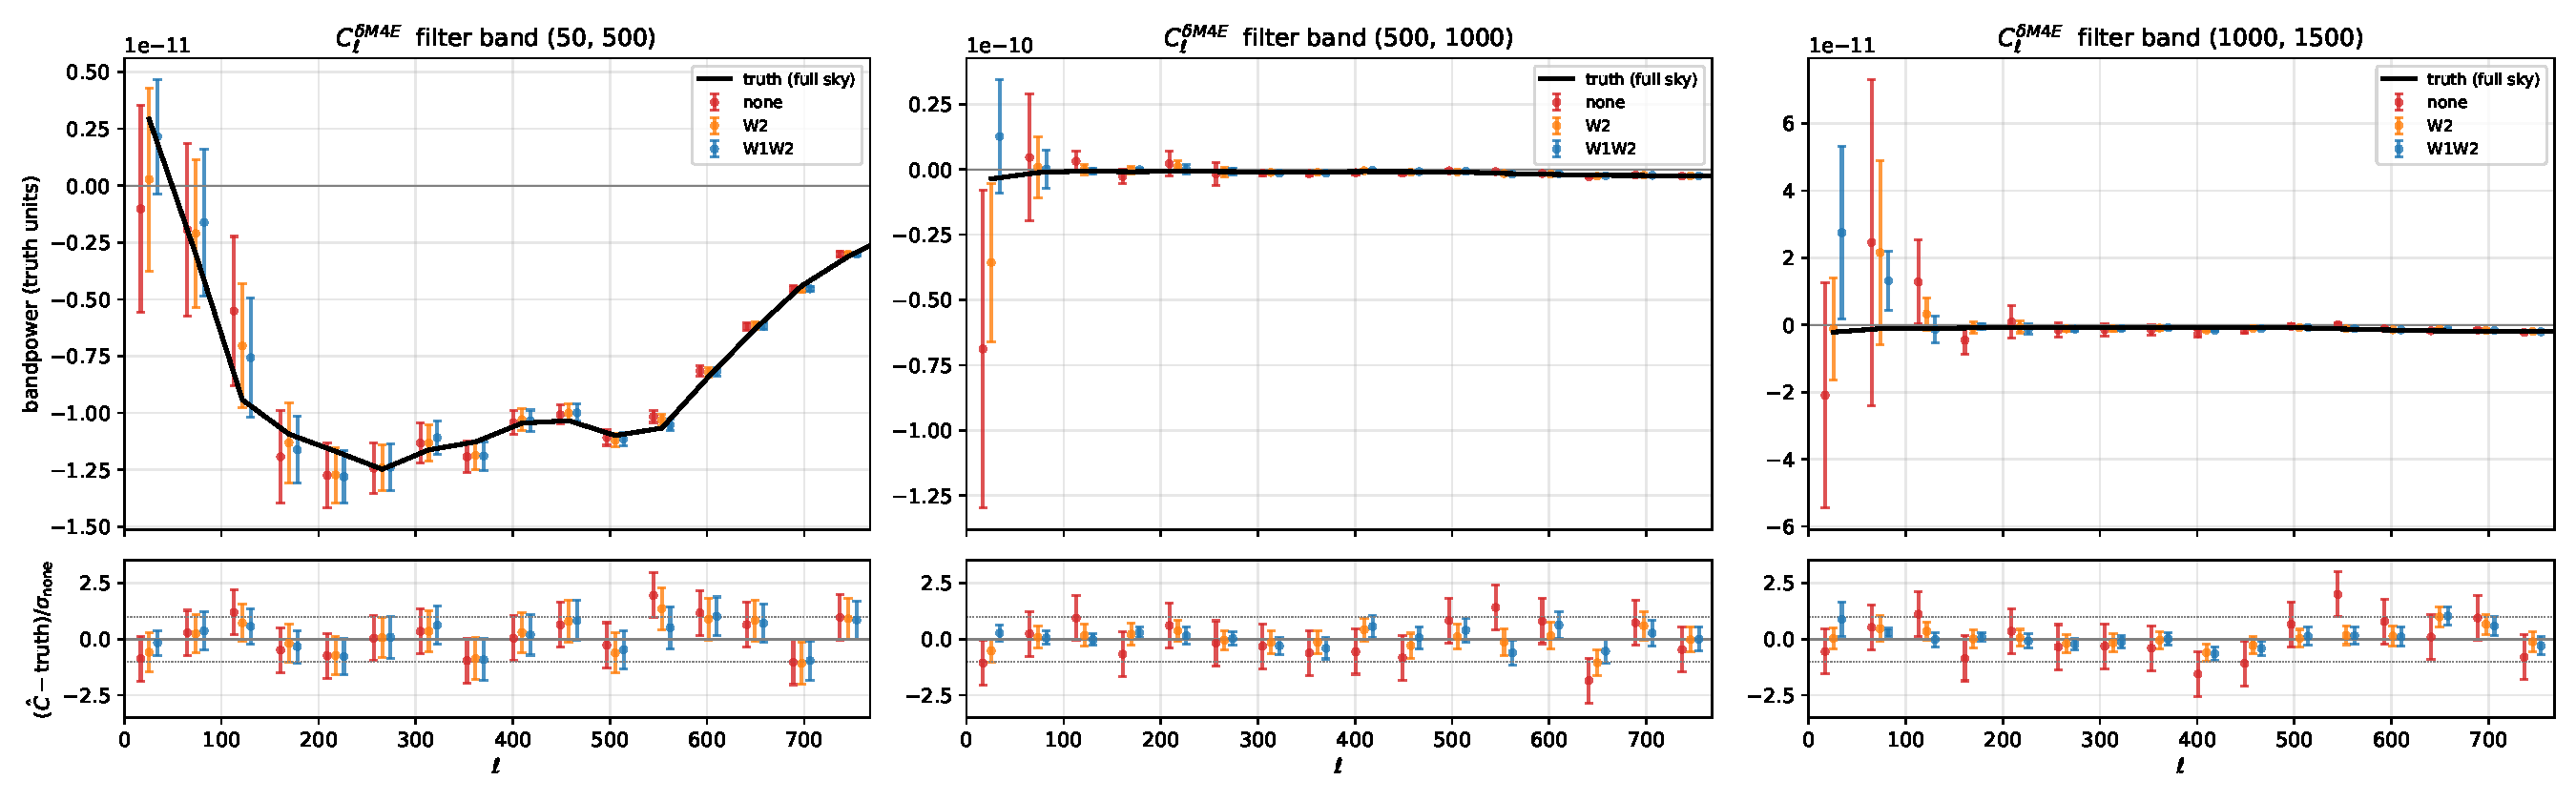
\includegraphics[width=\textwidth]{figures/cross_M4E_ns1024.pdf}
\caption{As \cref{fig:crossM0} for the spin-4 $E$-mode cross
$\hat C_\ell^{\dt M_{4E}}$ (no noise bias), corrected by $T^{\rm (A)}$.}
\label{fig:crossM4}
\end{figure}

\begin{figure}[p]
\centering
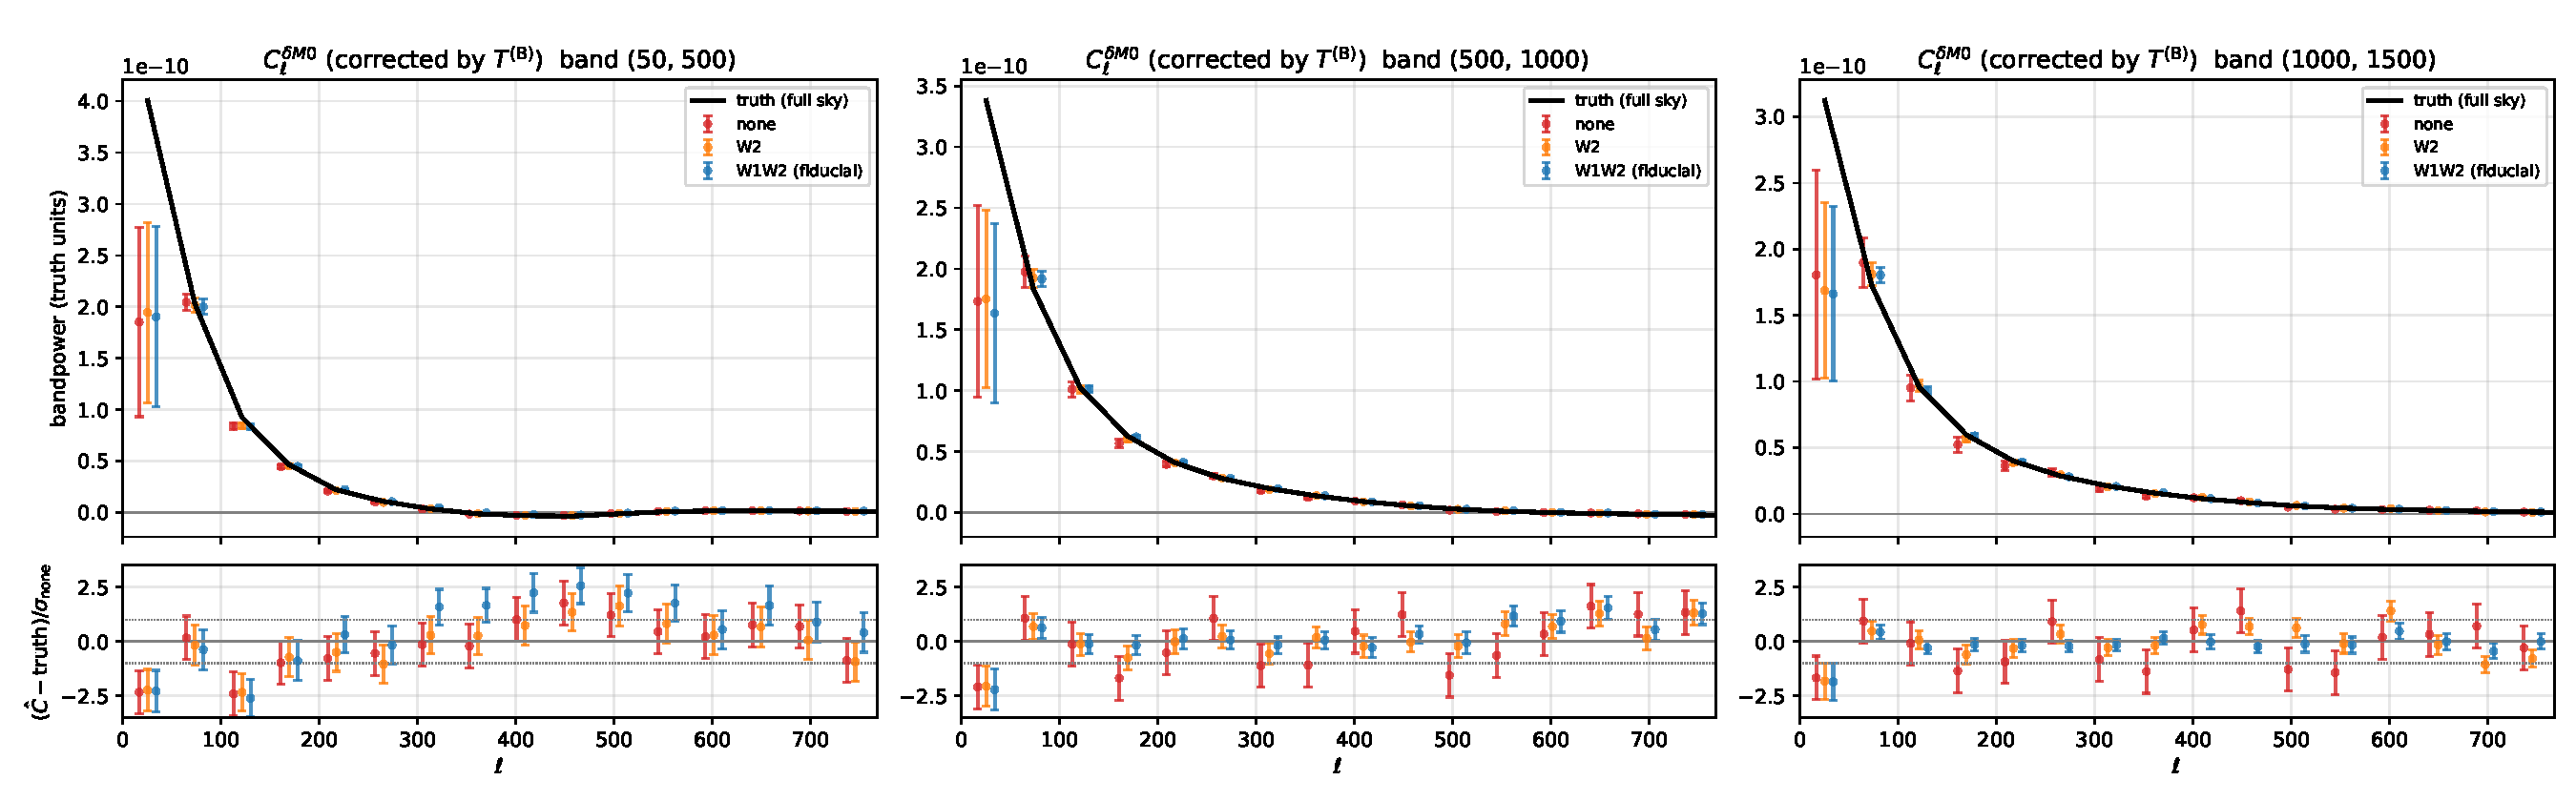
\includegraphics[width=\textwidth]{figures/cross_M0_predB_ns1024.pdf}
\caption{\textbf{Fiducial.} $\hat C_\ell^{\dt M_0}$ as \cref{fig:crossM0} but
corrected by the \emph{independent} analytic transfer $T^{\rm (B)}$ (predicted
from the survey window and power spectra, no signal-sim input).}
\label{fig:crossM0predB}
\end{figure}

\begin{figure}[p]
\centering
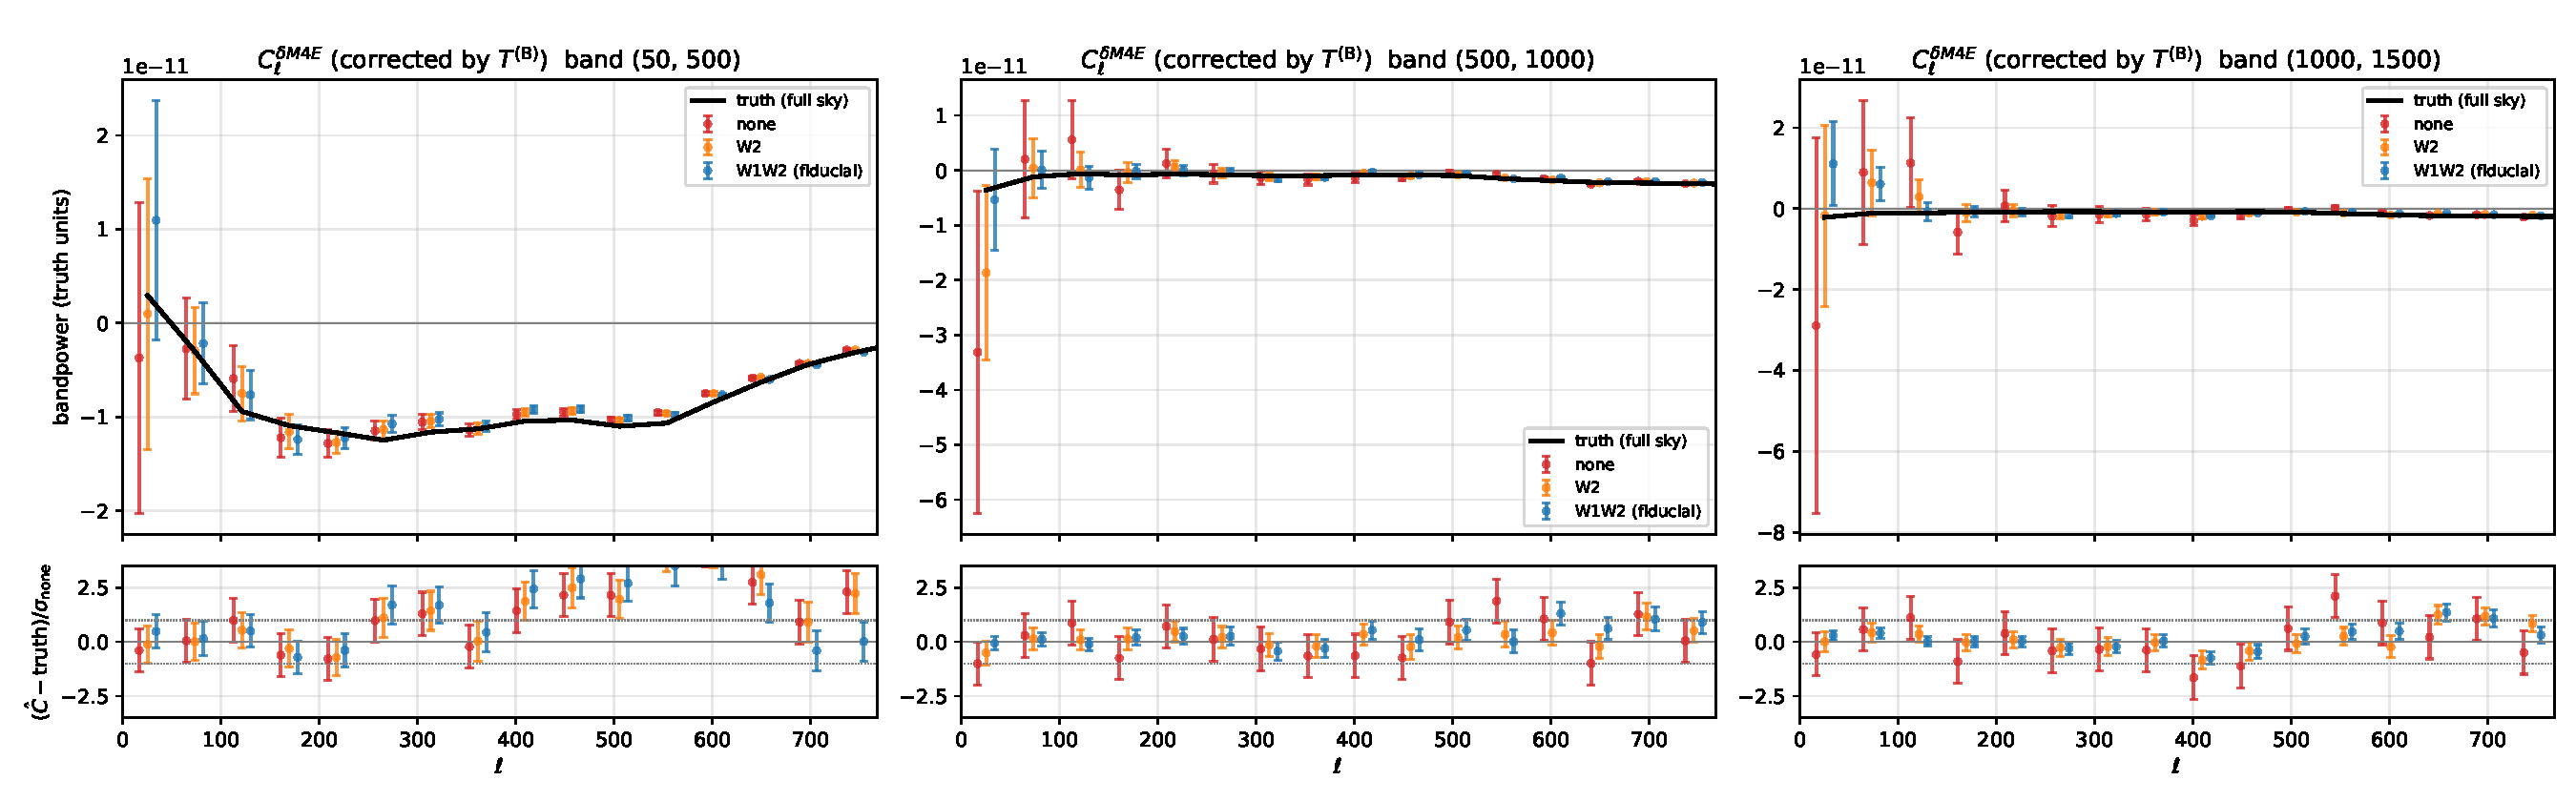
\includegraphics[width=\textwidth]{figures/cross_M4E_predB_ns1024.pdf}
\caption{As \cref{fig:crossM0predB} for the spin-4 cross
$\hat C_\ell^{\dt M_{4E}}$, corrected by the analytic $T^{\rm (B)}$.}
\label{fig:crossM4predB}
\end{figure}

\begin{figure}[p]
\centering
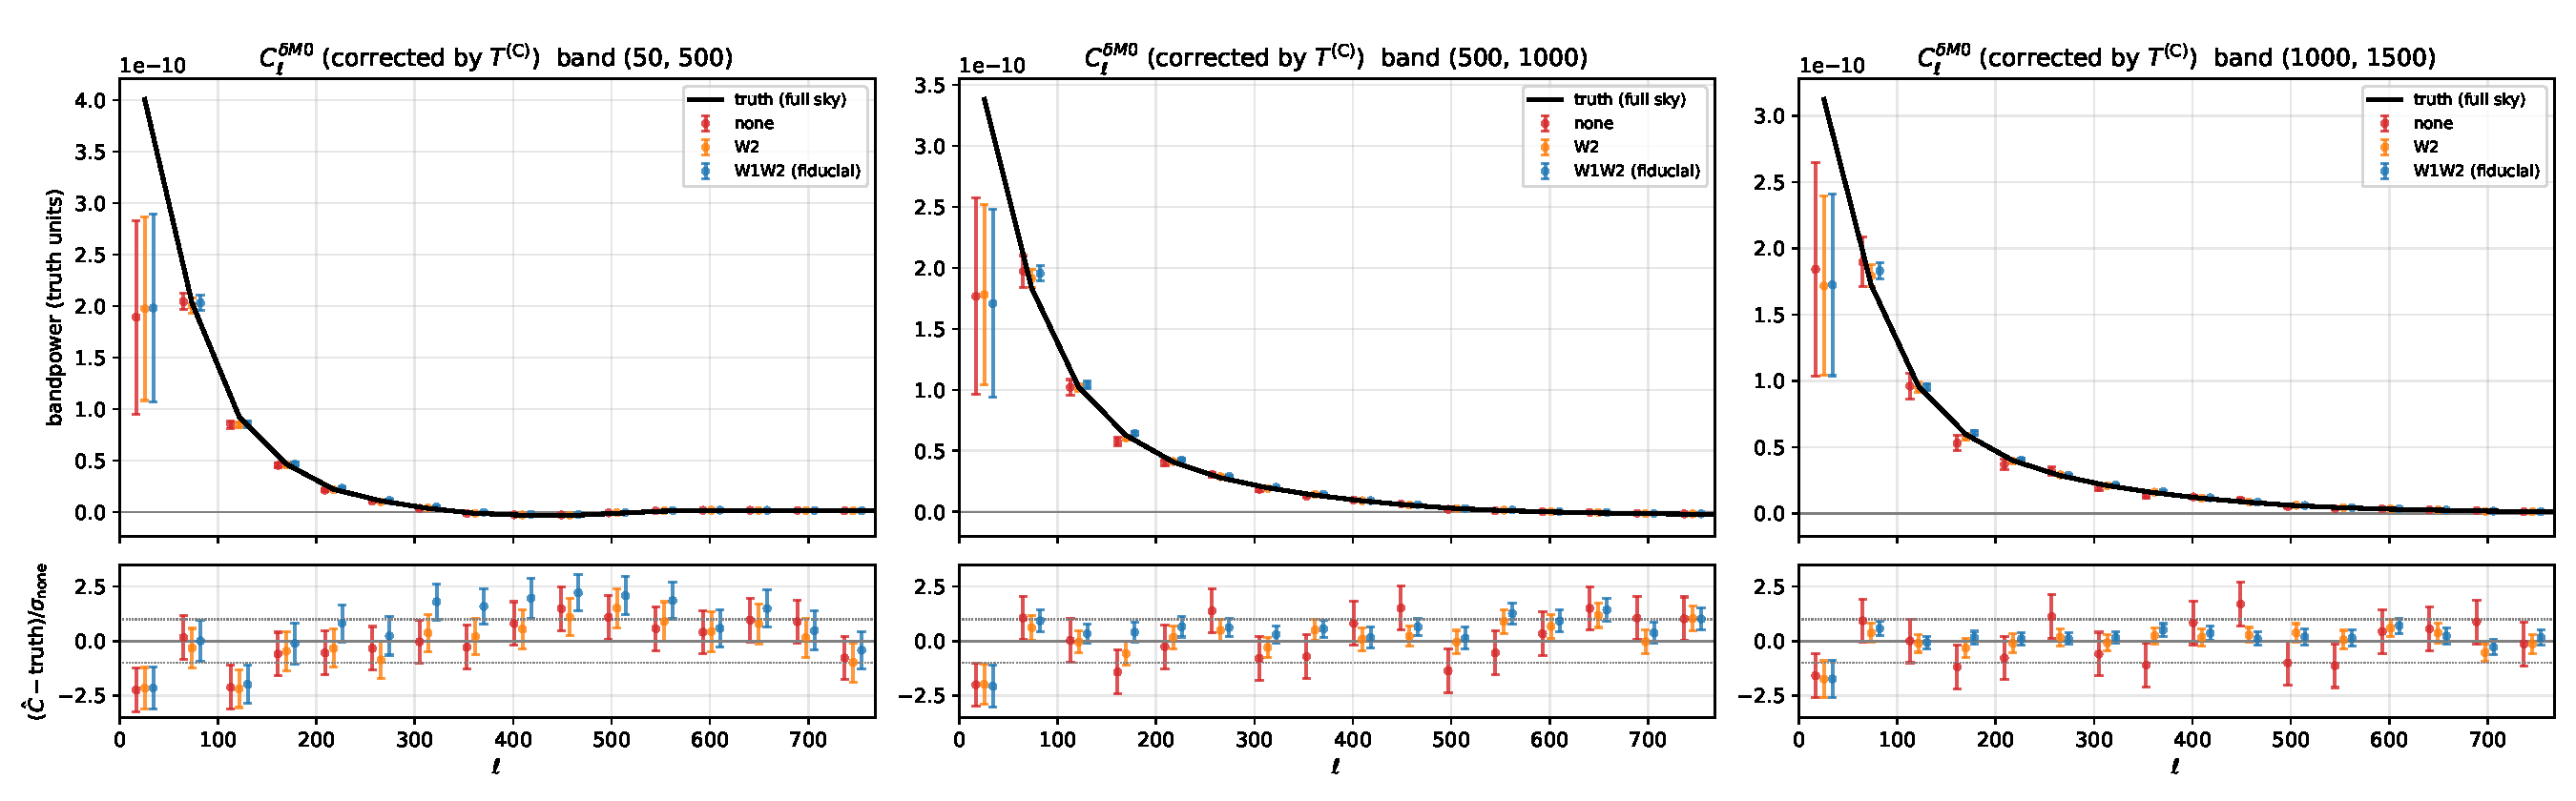
\includegraphics[width=\textwidth]{figures/cross_M0_predC_ns1024.pdf}
\caption{As \cref{fig:crossM0predB} but corrected by the \emph{closed-form}
analytic transfer $T^{\rm (C)}$ of \cref{eq:TC} (the Monte-Carlo--free
$g_{\rm edge}\times N_{\rm weight}$ factorization, constant within each band). The
bandpowers remain consistent with truth, matching the (B) result, which confirms
that the closed-form transfer is an adequate first-principles calibration in its
own right.}
\label{fig:crossM0predC}
\end{figure}

\begin{figure}[p]
\centering
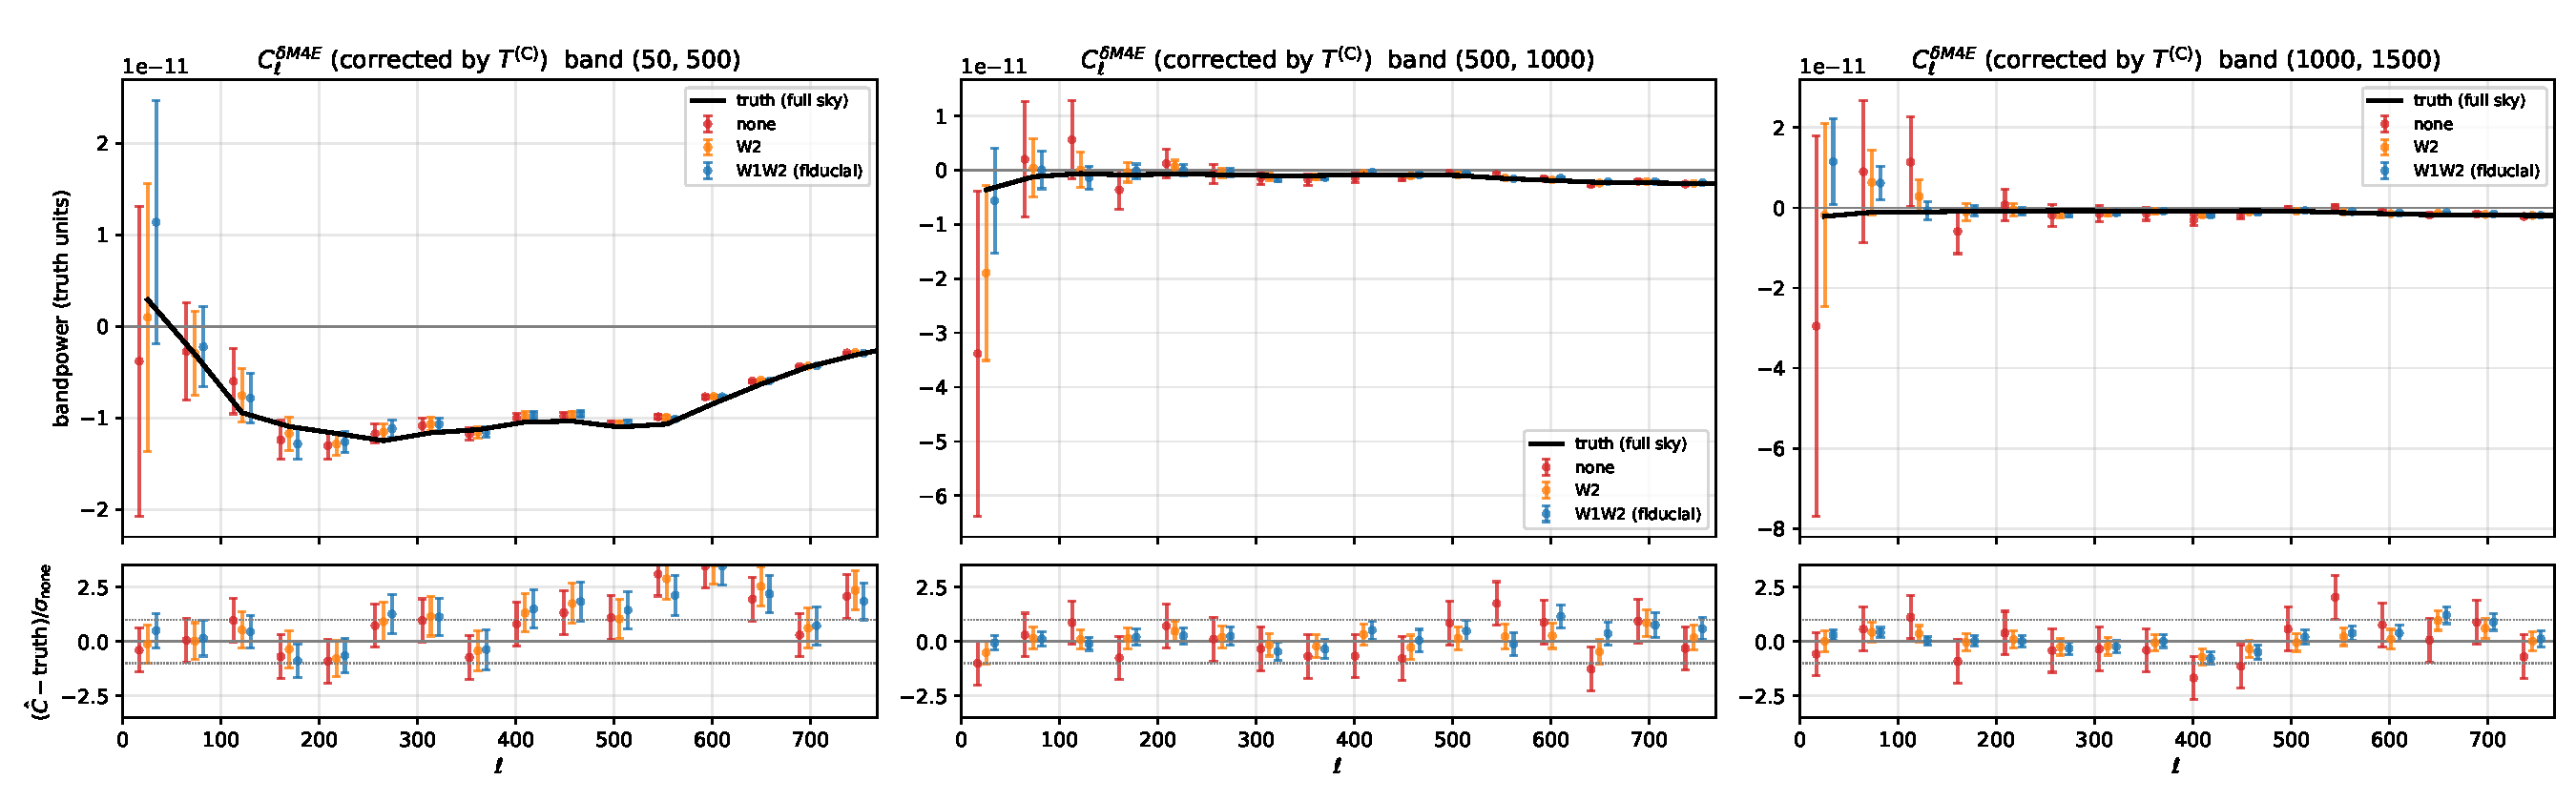
\includegraphics[width=\textwidth]{figures/cross_M4E_predC_ns1024.pdf}
\caption{As \cref{fig:crossM0predC} for the spin-4 cross
$\hat C_\ell^{\dt M_{4E}}$, corrected by the closed-form $T^{\rm (C)}$.}
\label{fig:crossM4predC}
\end{figure}

\begin{figure}[p]
\centering
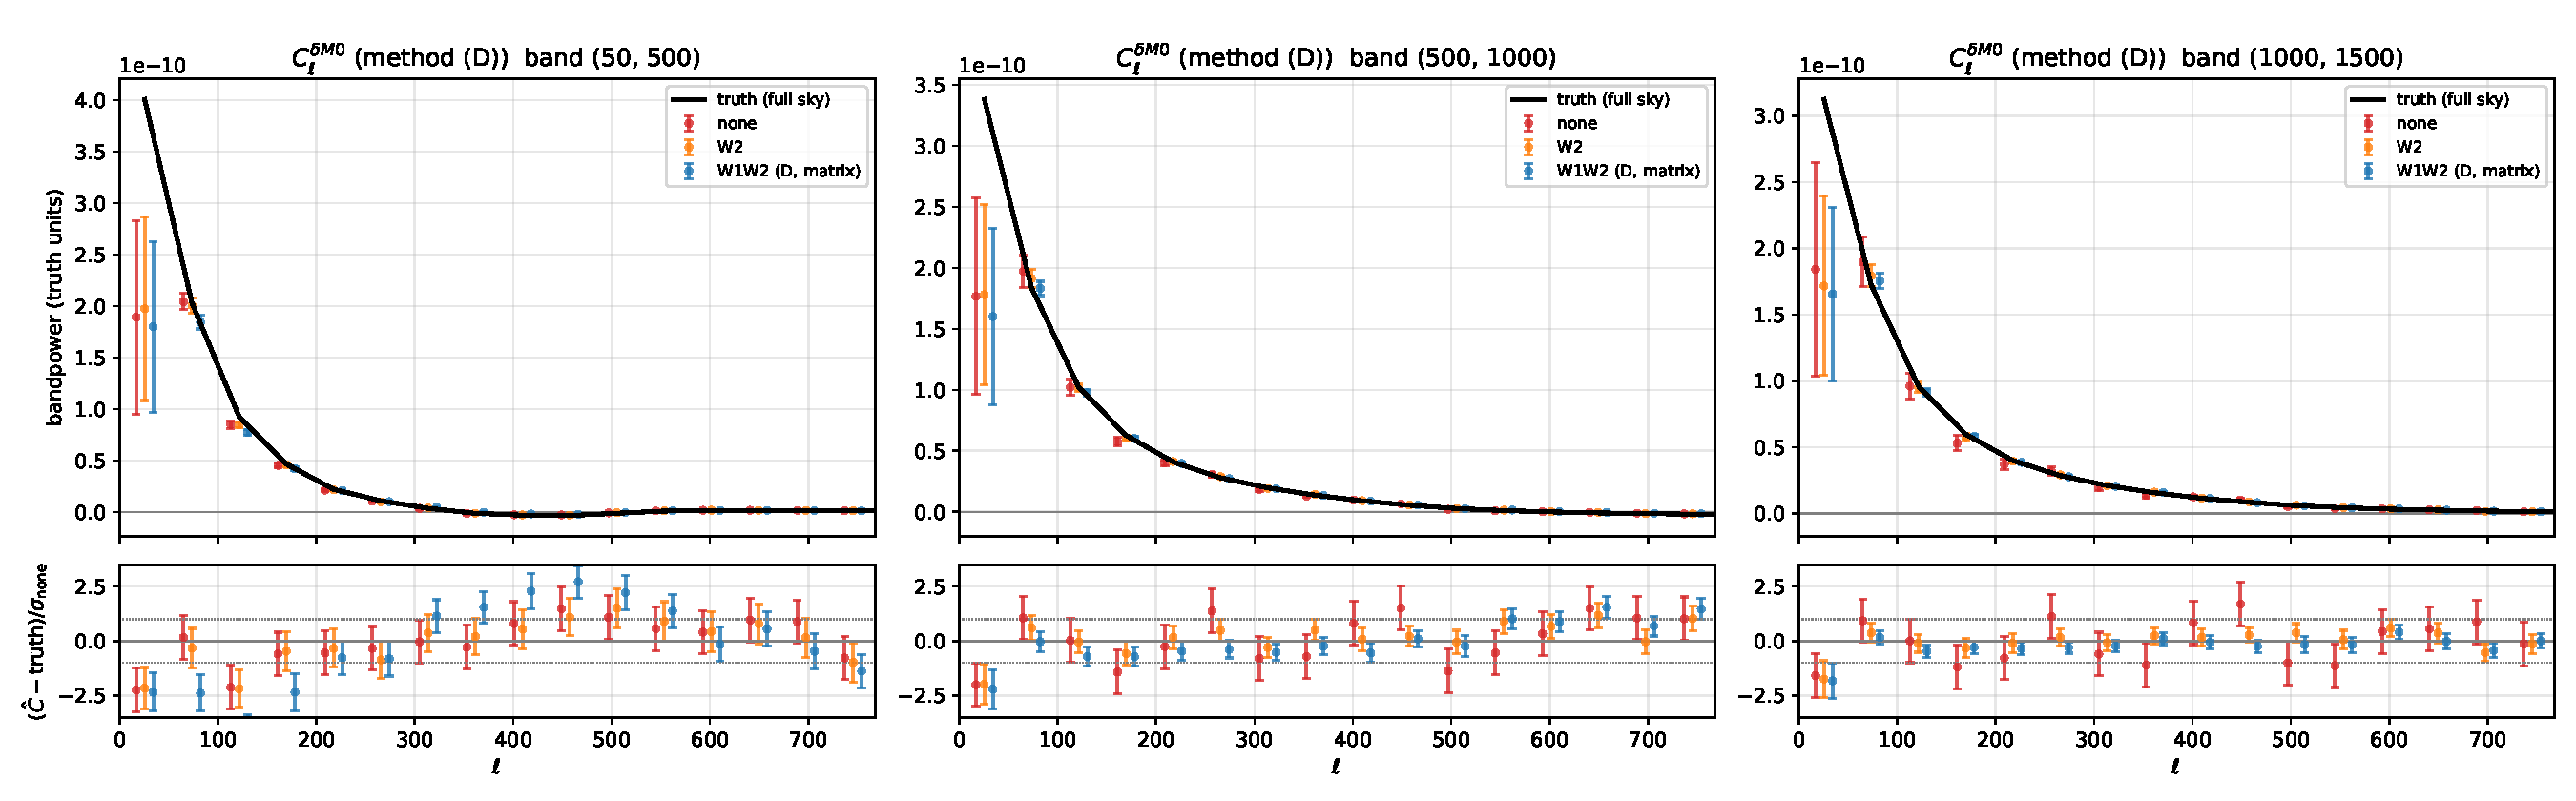
\includegraphics[width=\textwidth]{figures/cross_M0_predD_ns1024.pdf}
\caption{As \cref{fig:crossM0predB} but with the \textbf{W1W2} channel
calibrated by method (D), \cref{eq:TD}: the bandpowers are decoupled with the
mode-coupling matrix of the kernel-smoothed effective window
$\Wtwo{\rm m}\,(\kappa\star\Wone^2)$ of \cref{eq:wDsmooth}, which absorbs the
$\Wone$ modulation and the edge loss as a matrix --- \emph{no transfer
function is applied}. The \textbf{none}/\textbf{W2} schemes (for which (D)
reduces to the standard decoupling) are corrected by
$T^{\rm (C)}=g_{\rm edge}$ as before.}
\label{fig:crossM0predD}
\end{figure}

\begin{figure}[p]
\centering
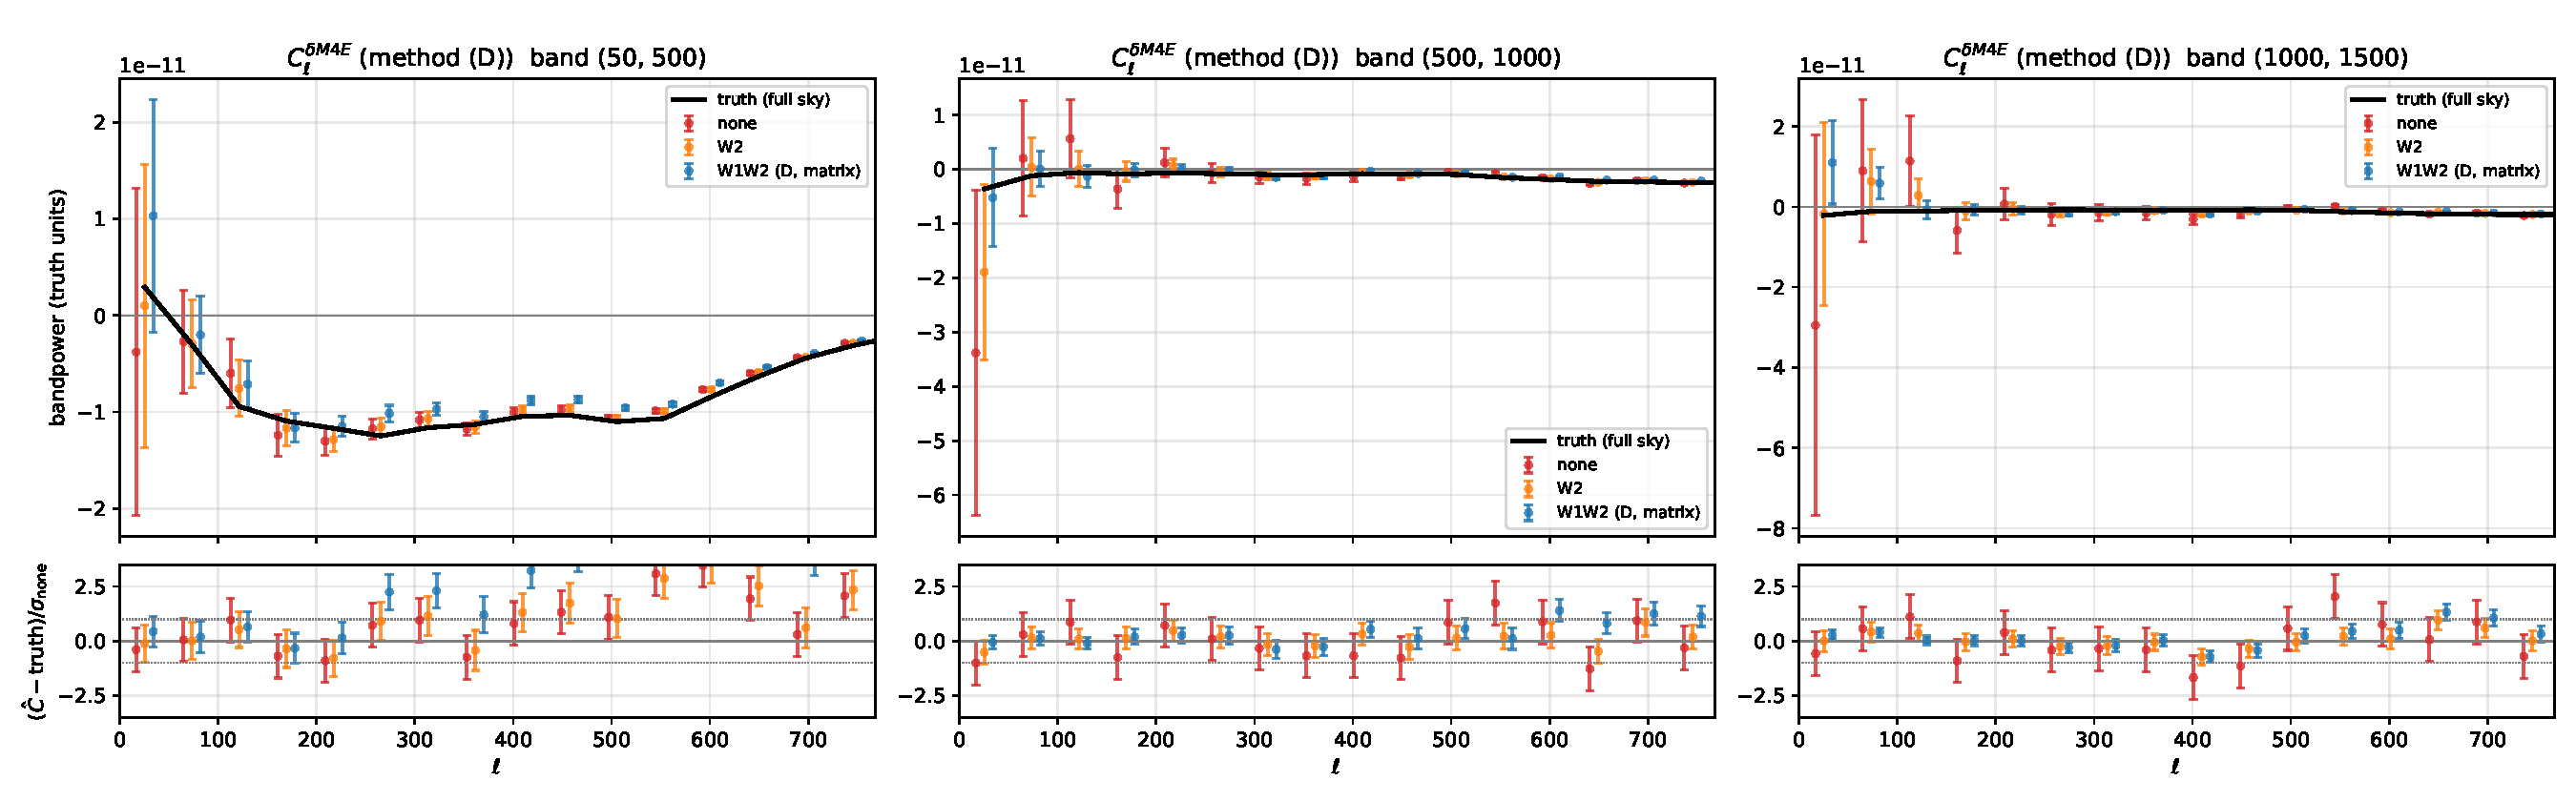
\includegraphics[width=\textwidth]{figures/cross_M4E_predD_ns1024.pdf}
\caption{As \cref{fig:crossM0predD} for the spin-4 cross
$\hat C_\ell^{\dt M_{4E}}$, with the \textbf{W1W2} channel matrix-decoupled
per method (D).}
\label{fig:crossM4predD}
\end{figure}

\subsection{Covariance cross-check}

Because the four footprints are equal-area and disjoint, the covariance of one
sample equals the NaMaster Gaussian (Knox-like) covariance for a single
footprint, which we evaluate from the on-the-fly $\dt\dt$, $M_0M_0$, $\dt M_0$
auto/cross spectra. The diagonal of the Gaussian covariance matches the
$400$-sample scatter (\cref{tab:cov}), validating the analytic error bars.

\begin{table}[h]
\centering
\begin{tabular}{lccc}
\toprule
band & none & W2 & W1W2\\
\midrule
$[50,500]$    & $0.97$ & $0.96$ & $0.98$\\
$[500,1000]$  & $0.93$ & $0.96$ & $1.00$\\
$[1000,1500]$ & $0.95$ & $268^{\dagger}$ & $1.00$\\
\bottomrule
\end{tabular}
\caption{Median ratio $\sqrt{\mathrm{diag}\,C_{\rm
Gauss}}/\sqrt{\mathrm{diag}\,C_{\rm sample}}$ of the NaMaster Gaussian error to
the $400$-sample scatter for the $M_0$ cross. The agreement is at the few-percent
level except for one configuration ($\dagger$): the unweighted-shear,
highest-band W2 weight $\propto1/(|K|^2\!\star n^2)^2$ is extremely peaked (the
band-$[1000,1500]$ noise spans more than a decade), which destabilises the
on-the-fly Gaussian-covariance inputs; the W1W2 scheme, which pre-whitens with
$\Wone=1/n^2$, is stable there ($1.00$). This affects only the analytic
cross-check, not the sample-covariance results.}
\label{tab:cov}
\end{table}

\Cref{fig:covcompare} compares the two error estimates directly: the
per-realization $\sigma(\hat C_\ell^{\dt M_0})$ from the $400$-realization scatter
(points) and from the NaMaster Gaussian covariance (lines) lie on top of each
other across all bands and schemes, except the single anomalous W2,
$[1000,1500]$ configuration (the high orange line in the right panel).

\begin{figure}[t]
\centering
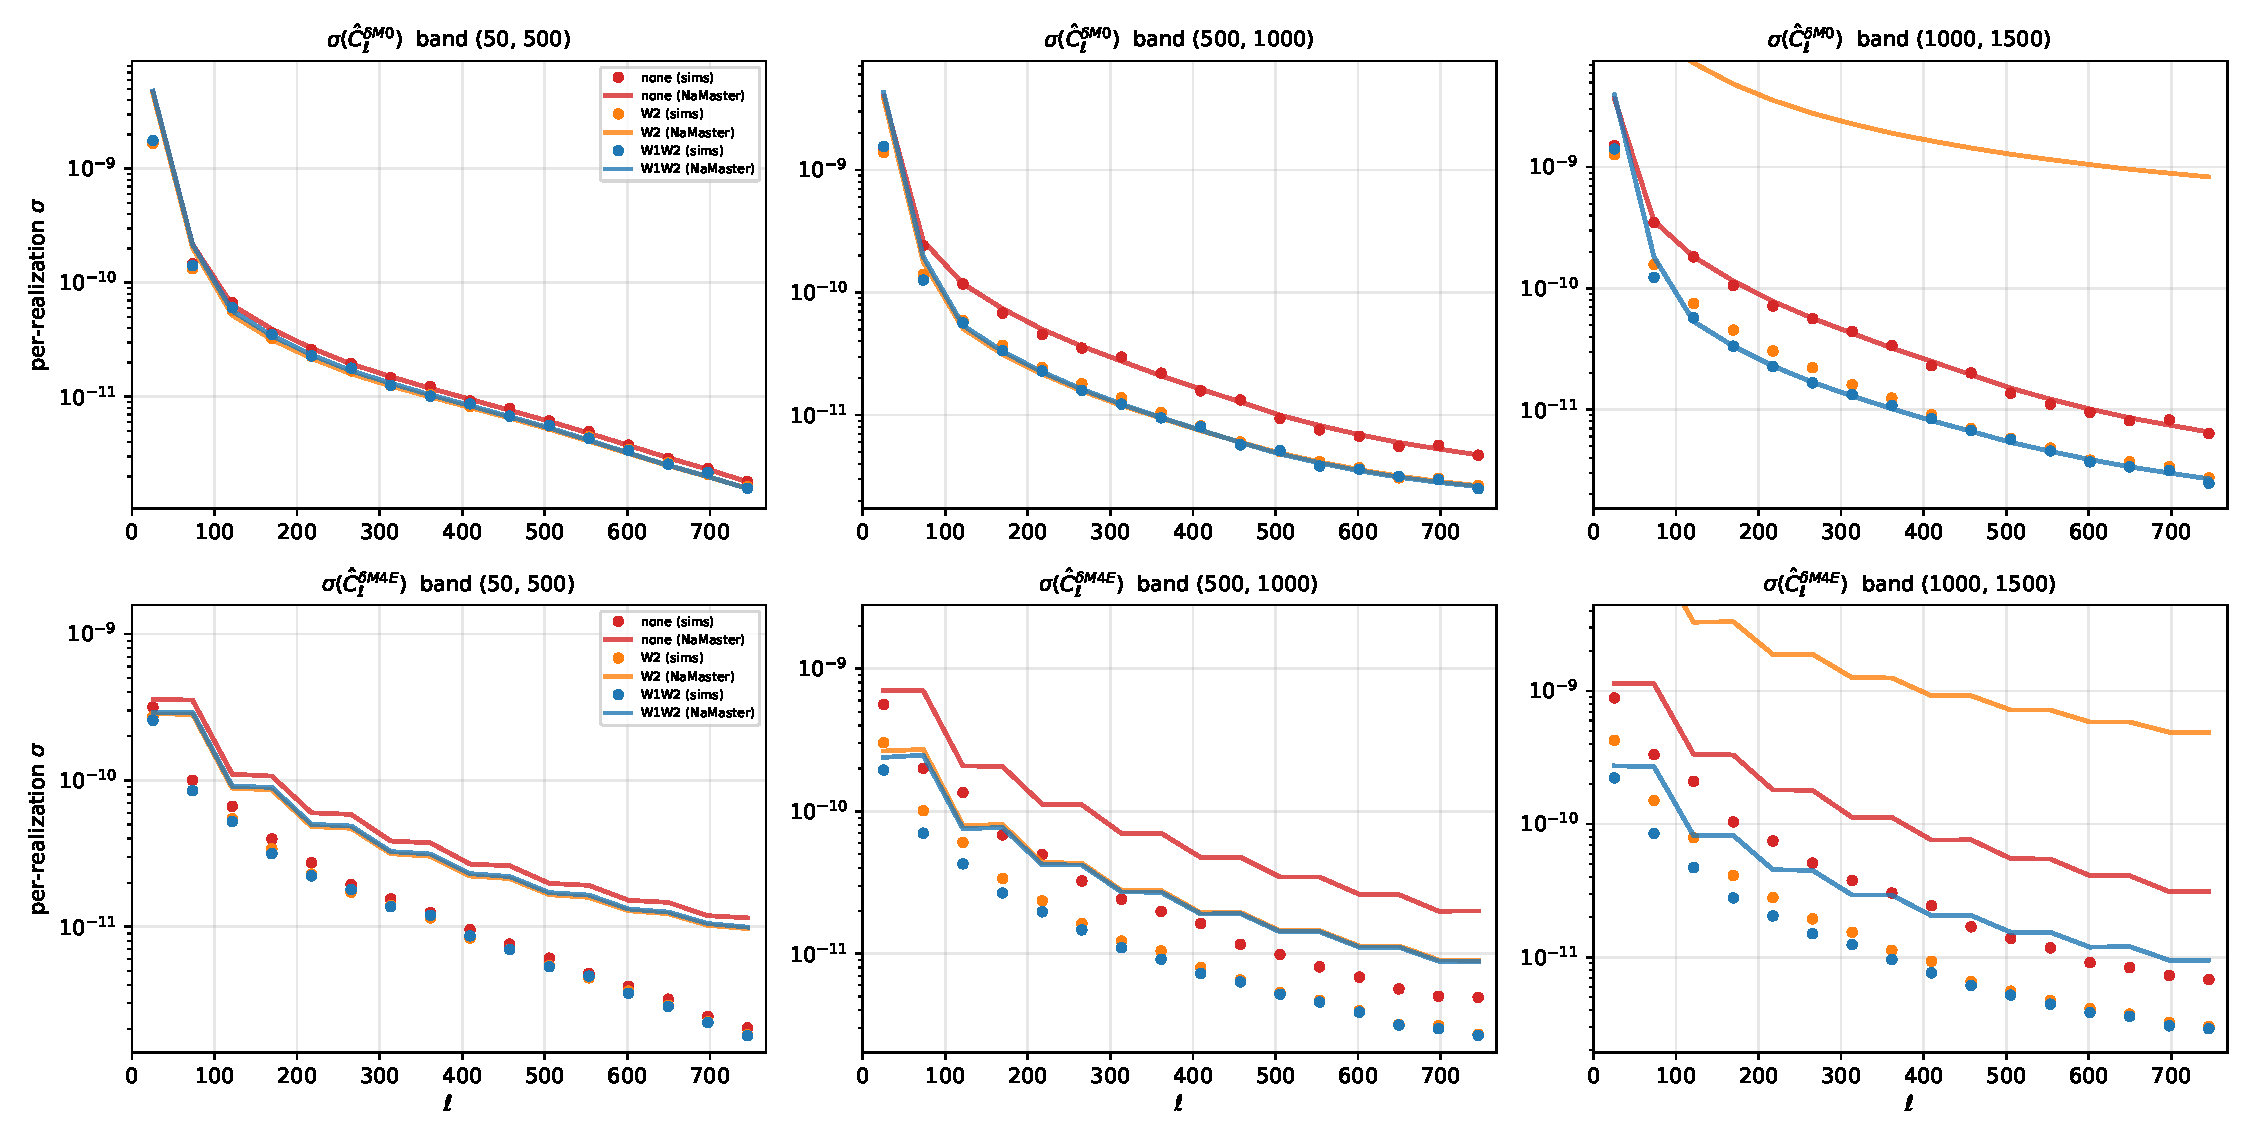
\includegraphics[width=\textwidth]{figures/cov_compare_ns1024.pdf}
\caption{Per-realization error $\sigma=\sqrt{\mathrm{diag}\,C}$ from the
$400$-realization sample scatter (points) versus the NaMaster Gaussian covariance
(lines), for the three schemes and three bands, for $M_0$ (top) and $M_{4E}$
(bottom). For the spin-0 $M_0$ cross the two agree to a few percent
(cf.\ \cref{tab:cov}; the lone outlier is the orange line in $[1000,1500]$, the
peaked unwhitened-W2 weight). For the spin-4 $M_{4E}$ cross the Gaussian estimate
runs parallel to the sample $\sigma$ (the $\ell$-shape and scheme ordering match)
but high by a near-constant factor $\approx3$: the
$f_{\rm sky}=\langle w^2\rangle$ deconvolution of the input auto-spectra is cruder
for spin-weighted fields, whose mask coupling loses more power than the scalar
$\langle w^2\rangle$ captures. In both channels the
error drops from \textbf{none} (red) through \textbf{W2} (orange) to \textbf{W1W2}
(blue) in the noise-dominated bands --- the SNR gain of \cref{tab:chi2}. The
sample covariance (which is what the analysis uses) is robust for both.}
\label{fig:covcompare}
\end{figure}

\Cref{fig:cormat} shows the correlation matrices of the $400$-realization
covariance: they are strongly diagonal-dominant for both $M_0$ and $M_{4E}$ in
all bands (off-diagonals $|r|\lesssim0.25$), with only a mild anti-correlation
between the two lowest-$\ell$ bandpowers (the ill-conditioned largest scales on
the $\sim11\%$ footprint). The near-diagonal covariance justifies the diagonal
$\chi^2$ used above.

\begin{figure}[t]
\centering
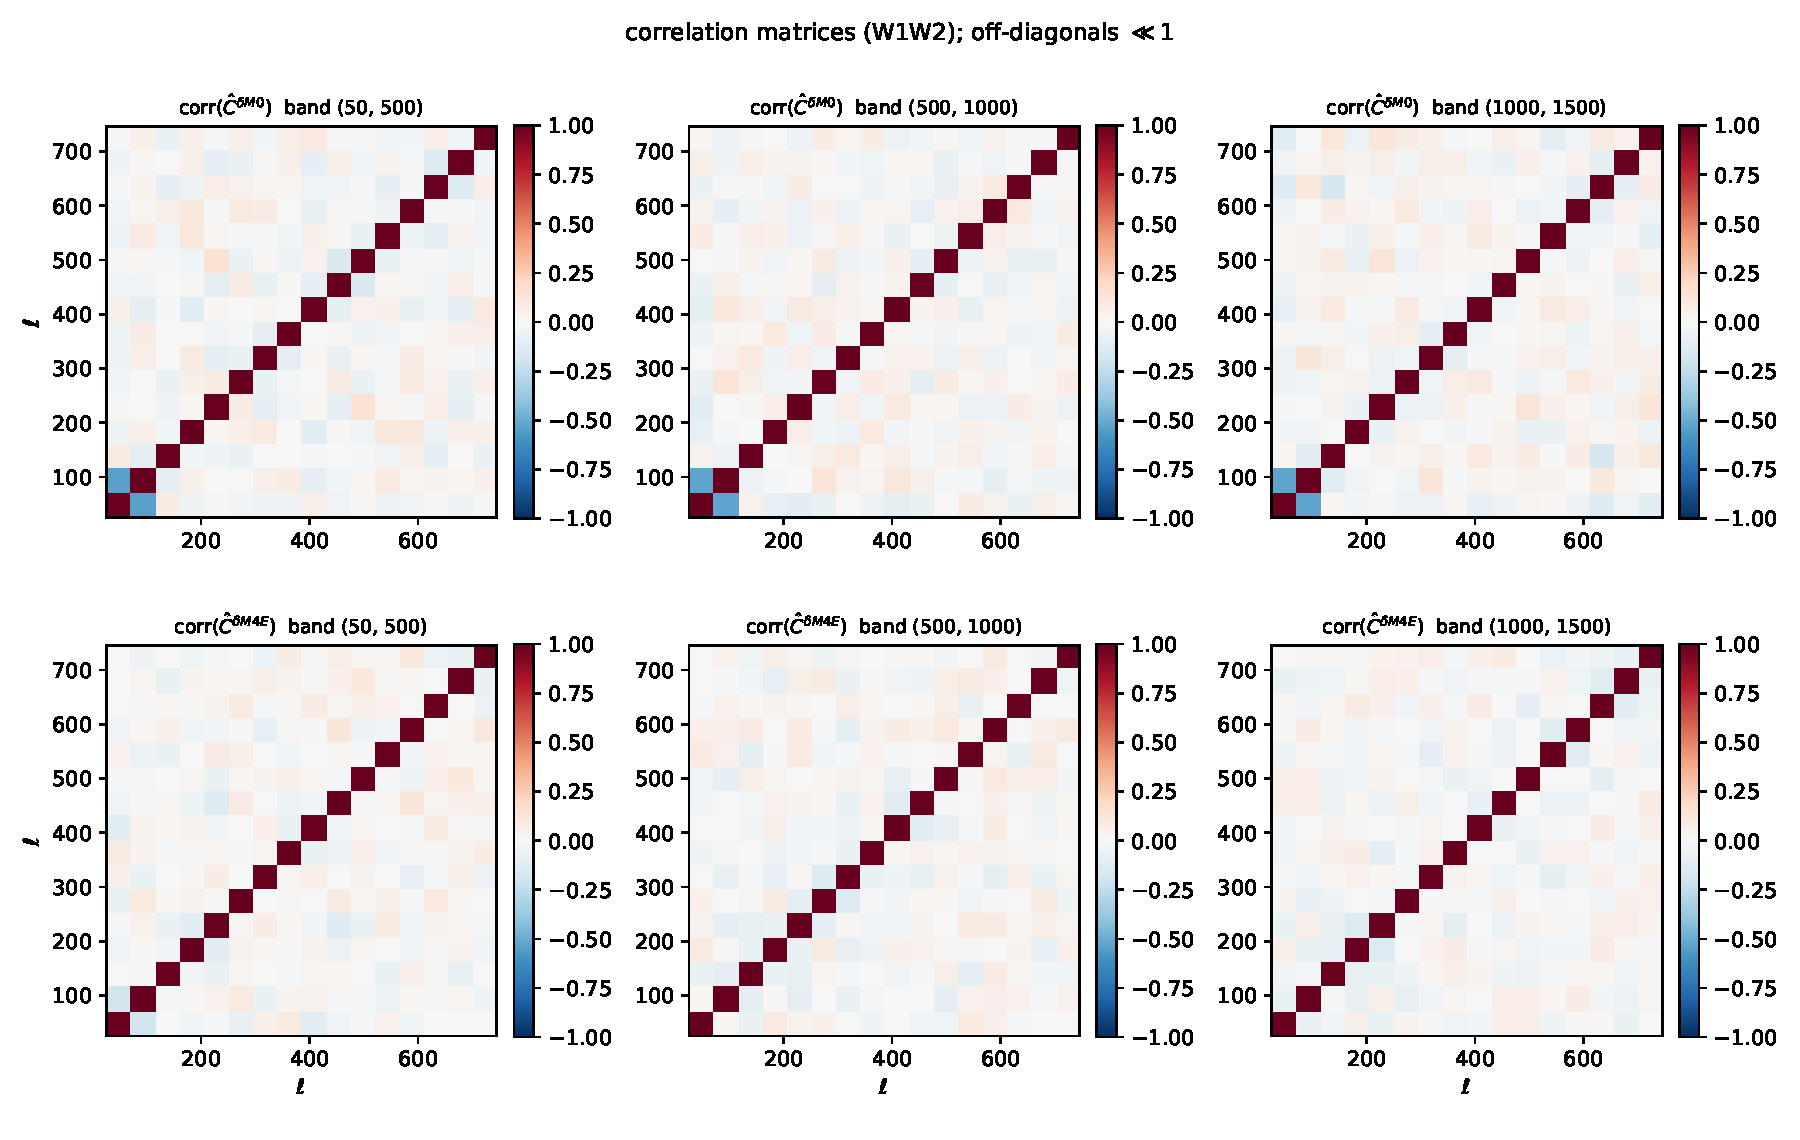
\includegraphics[width=\textwidth]{figures/cormat_ns1024.pdf}
\caption{Correlation matrices $C_{\ell\ell'}/\sqrt{C_{\ell\ell}C_{\ell'\ell'}}$ of
the $400$-realization covariance for the W1W2 scheme, for $M_0$ (top) and
$M_{4E}$ (bottom) in the three bands. The matrices are nearly diagonal; the only
visible off-diagonal feature is a mild anti-correlation of the two largest-scale
bandpowers.}
\label{fig:cormat}
\end{figure}

\subsection{Signal-to-noise and the gain from weighting}

In the low band $[50,500]$ the cross variance is signal-dominated (the shape
noise contributes $\sim1\%$ of $\Var[\hat C_\ell^{\dt M_0}]$), so optimal
weighting yields no gain --- consistent with the note, whose weights minimize
the noise-dominated term. In the higher, noise-dominated bands the inverse
variance weighting reduces the error: \cref{fig:snr} compares the per-bandpower
error of the three schemes, and the detection SNR in \cref{tab:chi2} rises
substantially from \textbf{none} to \textbf{W2} to \textbf{W1W2}: for $M_0$,
$2.3\to4.2\to5.0$ in $[500,1000]$ and $1.9\to4.1\to5.6$ in $[1000,1500]$ --- a
factor of $2.2$--$2.9$ improvement in significance, of which most comes from the
post-square weight $\Wtwo$ and a further $\sim20$--$35\%$ from adding the
pre-filter $\Wone$. The spin-4 $M_{4E}$ cross shows the same pattern
($0.5\to1.2$ in the top band). In the signal-dominated band $[50,500]$ the gain
is marginal ($2.9\to3.2$), as expected.

\begin{figure}[t]
\centering
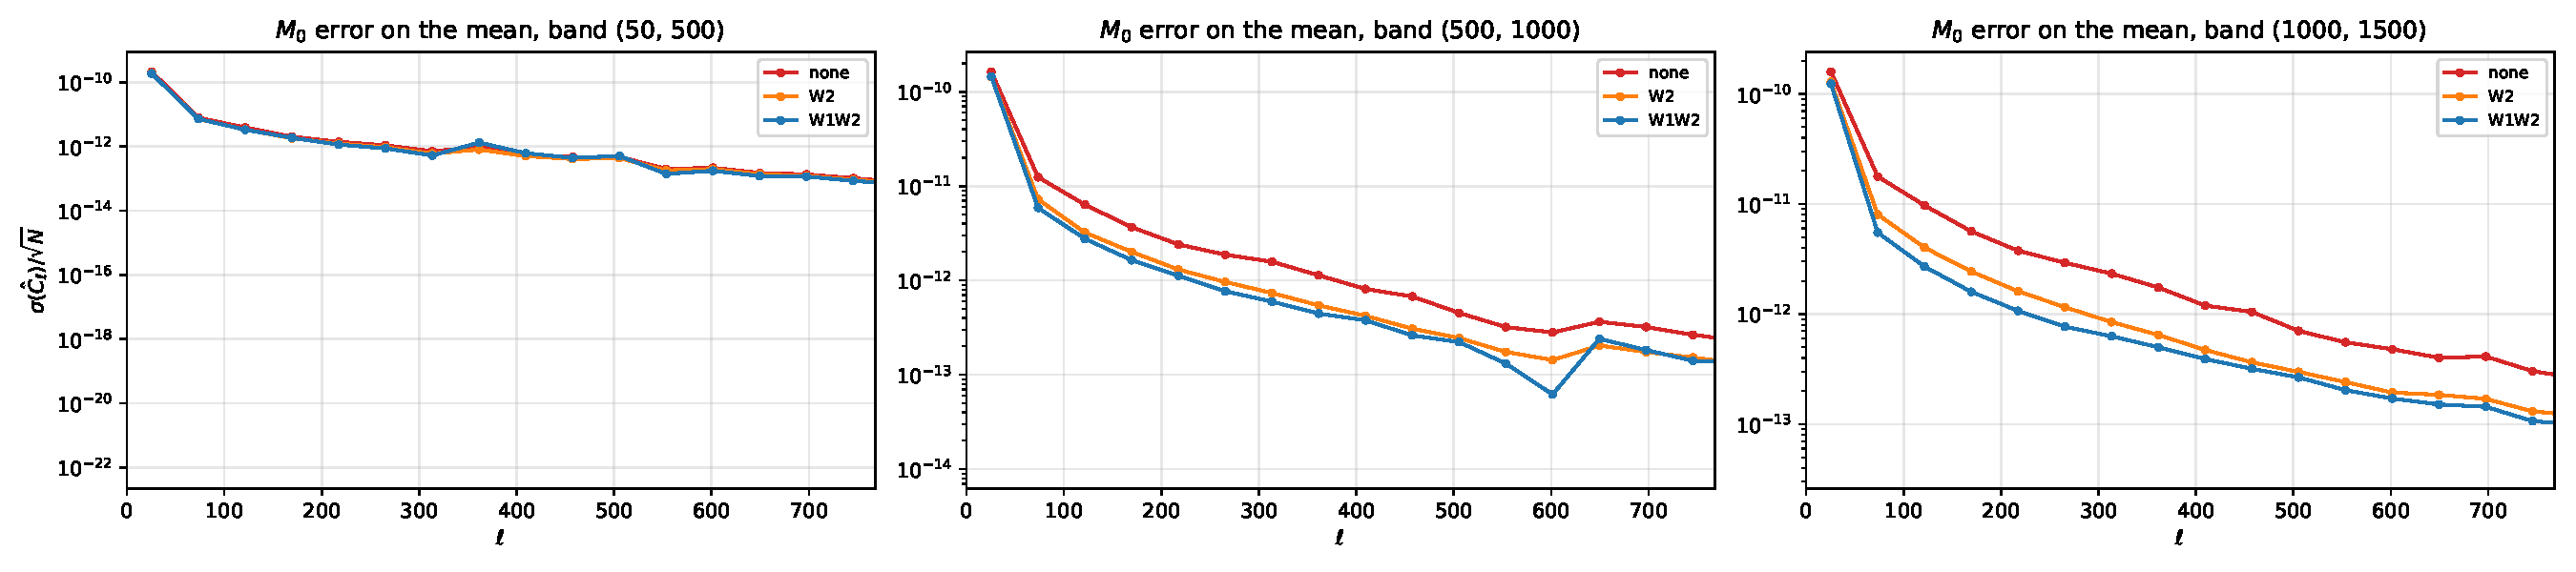
\includegraphics[width=\textwidth]{figures/snr_M0_ns1024.pdf}
\caption{Per-bandpower error on the mean of $\hat C_\ell^{\dt M_0}$ for the
three schemes. In the noise-dominated bands, optimal weighting (W2, W1W2)
lowers the error relative to the unweighted (none) estimator.}
\label{fig:snr}
\end{figure}

\section{Code overview}

The estimator is packaged as the installable Python module \texttt{fsb\_ssg}
(\emph{Filtered-Square Bispectrum: shear--shear--galaxy}); this validation lives
in \texttt{science/} of the same repository and runs with pymaster~2.7 and
healpy~1.19. The generic estimator is in \texttt{src/fsb\_ssg/}; the
survey-specific adapter \texttt{science/pipeline/simlib.py} binds it to the
simulation configuration and map IO, so the physics lives in one place. The
pipeline is staged by \texttt{science/pipeline/run\_pipeline.sh}
(\texttt{FSB\_NSIDE}, \texttt{FSB\_SIM\_DIR}; masks run in parallel at
$N_{\rm side}\ge1024$):
\begin{description}
\item[\texttt{fsb\_ssg} (library)] core library: the inhomogeneous
noise model, $\Wone$/$\Wtwo$ construction (\cref{eq:W2}), the filtered-square
step, the \texttt{bl2beam} $|K|^2$ noise-bias template, the squeezed-response
kernel $\kappa$ (\cref{eq:kappa}), and the NaMaster spin-0$\times$spin-0 ($M_0$)
and spin-0$\times$spin-4 ($M_{4E}$) decoupled cross-spectra. Unit-tested on
synthetic maps via GitHub Actions; cached map IO is provided by the
\texttt{simlib} adapter.
\item[\texttt{build\_cache.py}] degrade and cache the input maps to the working
resolution (skipped at $N_{\rm side}=1024$, where the maps are native).
\item[\texttt{ground\_truth.py}] full-sky, noise-free, unit-weight ground truth
(through NaMaster with a unit mask, apples-to-apples).
\item[\texttt{run\_masked.py} + \texttt{combine\_masks.py}] the $100\times4$
masked, noisy run for the three schemes and the signal-only channel (for
$T^{\rm (A)}$); parallel per mask, then combined.
\item[\texttt{analyze.py}] the two unbiasedness $\chi^2$ tests, the
$T^{\rm (A)}$-corrected cross-spectra, the SNR comparison, the correlation
matrices, and the table data.
\item[\texttt{predict\_transfer.py}] the analytic transfer (\cref{app:transfer}):
methods (B) Gaussian-MC and (C) closed form, the three-method comparison, and the
fiducial $T^{\rm (B)}$-corrected cross-spectra.
\item[\texttt{nmt\_covariance.py}] the NaMaster Gaussian covariance versus the
sample scatter, for $M_0$ and $M_{4E}$.
\item[\texttt{method\_d.py}] the method-(D) mode-coupling calibration
(\cref{eq:TD}): the dummy-window ($\Wtwo{\rm m}\Wone^2$) coupling matrices, the
exact linear re-decoupling of the stored bandpowers, its validation, and the
(D) figures.
\end{description}

\appendix

\section{Analytic transfer function}\label{app:transfer}

The transfer function quantifies why the masked, weighted \emph{filter-then-square}
estimator differs from the full-sky \emph{filter-then-square} ground truth for the
same sky. For a Gaussian shear field it is calculable from the mask, the weights
$\Wone,\Wtwo$, the filter, and the shear power spectrum $C^{\gamma\gamma}_\ell$.

\paragraph{Filtered-shear kernel.}
Let $\xi=F[\Wone\bm\gamma]$ be the bandpass-filtered (weighted) shear, with
real-space bandpass kernel $K(\theta)=\mathrm{bl2beam}(f_\ell)$. Its full-sky,
homogeneous two-point function is
\begin{equation}
\rho(\theta)=\E[\xi(\nv)\xi^*(\nv')]
=\sum_\ell\frac{2\ell+1}{4\pi}f_\ell^2\,C^{\gamma\gamma}_\ell\,P_\ell(\cos\theta),
\qquad \E[M_0]=\rho(0).
\end{equation}

\paragraph{Squeezed response.}
The shear--shear--density signal is the response of the small-scale shear power to
the large-scale lens density: $C^{\gamma\gamma}_\ell\to
C^{\gamma\gamma}_\ell[1+b_\phi\,\dt(\nv)]$ across the band. To linear order the
$\dt$-correlated part of $M_0$ is
\begin{equation}
\delta M_0(\nv)=b_\phi\!\int\!\!\int K(\nv,a)K^*(\nv,b)\,\Wone(a)\Wone(b)\,
C^{\gamma\gamma}(a\!\cdot\!b)\,\dt(a)\,\diff a\,\diff b\;+\;(a\!\leftrightarrow\!b),
\end{equation}
where $\Wone$ carries the binary mask. Doing the inner integral,
$\int K^*(\nv,b)C^{\gamma\gamma}(a\!\cdot\!b)\diff b$ has harmonic coefficients
$f_\ell C^{\gamma\gamma}_\ell$, so
\begin{equation}
\boxed{\;\delta M_0(\nv)=2b_\phi\,[\kappa\star(\Wone^2\dt)](\nv),\qquad
b^\kappa_\ell=\mathrm{beam2bl}\!\big[\mathrm{bl2beam}(f_\ell)\cdot
\mathrm{bl2beam}(f_\ell C^{\gamma\gamma}_\ell)\big].\;}
\label{eq:kappa}
\end{equation}
For a white band $C^{\gamma\gamma}_\ell=P_0$ this reduces to
$b^\kappa_\ell=P_0\,\mathrm{beam2bl}[\,|K(\theta)|^2]$, i.e.\ the squared-kernel
$|K|^2$ of the optimal-weights note (its noise template, with $n^2\!\to\!P_0$).
The shear power enters only through the \emph{shape} of $\kappa$ (its width within
the band); the response amplitude $b_\phi$ cancels below.

\paragraph{Transfer.}
Full sky with $\Wone=1$ gives the truth response $\delta M_0^{\rm t}=2b_\phi
\,\kappa\star\dt$, so $\langle\delta M_0^{\rm t}\dt\rangle_\ell=2b_\phi
b^\kappa_\ell C^{\dt\dt}_\ell$. NaMaster already removes the cross mode-coupling
of the $(\Wtwo\,\text{mask},\,\text{mask})$ weights, so the residual transfer is
the field-level window relating the constructed response $\kappa\star(\Wone^2\dt)$
to the truth $\kappa\star\dt$:
\begin{equation}
T_\ell=\frac{\big\langle\,\mathrm{decouple}_{\Wtwo{\rm m}}\,
\mathrm{pseudo}C_\ell[(\Wtwo\,{\rm m})\,\kappa\star(\Wone^2\dt),\ {\rm m}\,\dt]\big\rangle}
{\big\langle\,\mathrm{decouple}_{1}\,
\mathrm{pseudo}C_\ell[\kappa\star\dt,\ \dt]\big\rangle},
\label{eq:Tdef}
\end{equation}
independent of $b_\phi$ and of the normalization of $\kappa$.

\paragraph{Density assumption and weight contraction.}
We treat $\delta_{\rm src}$ as an externally \emph{fixed survey window}: it sets
the depth and hence the noise and the weights $\Wone,\Wtwo$, which are therefore
deterministic maps (like the mask). The lens density $\dt$ --- at a different
redshift --- is the random probe, taken uncorrelated with the window,
$\delta_{\rm src}\perp\dt$. The prediction thus uses only the spectra
$C^{\gamma\gamma}$ (via $\kappa$) and $C^{\dt\dt}$ (the probe), with $\dt$ drawn
from its spectrum; it never uses the lens map. Because $\Wone^2$ is fixed and
independent of $\dt$, the response $\kappa\star(\Wone^2\dt)$ is linear in $\dt$
and the transfer is a functional of $C^{\dt\dt}_\ell$ and the survey maps alone.

\paragraph{Four evaluations.}
\begin{itemize}
\item[(A)] \emph{Measured}: from the $400$ noise-free signal realizations of the
main run (these use the \emph{real}, weakly correlated $\delta_{\rm src}$ and
$\dt$).
\item[(B)] \emph{Gaussian Monte-Carlo}: a fixed $\delta_{\rm src}$ window
$\to$ fixed $\Wone,\Wtwo$; draw Gaussian $\dt$ from $C^{\dt\dt}_\ell$; propagate
$\kappa\star(\Wone^2\dt)$ through the identical NaMaster decoupling and average.
\item[(C)] \emph{Closed form (no Monte-Carlo)}:
\begin{equation}
\boxed{\;T_\ell^{\rm (C)}=g_{\rm edge}\times N_{\rm weight},\quad
g_{\rm edge}=\frac{\langle\kappa\star{\rm m}\rangle_{\rm m}}{\langle{\rm m}\rangle_{\rm m}},\quad
N_{\rm weight}=\frac{\langle\Wtwo\,{\rm m}\,\Wone^2\rangle}{\langle\Wtwo\,{\rm m}\rangle}\;}
\label{eq:TC}
\end{equation}
\item[(D)] \emph{Mode-coupling matrix}: decouple the measured pseudo-spectrum
with the NaMaster coupling matrix of an effective window carrying the weight
modulation (\cref{eq:TD} below); with the kernel-smoothed window
$w_{\rm D}=\Wtwo{\rm m}\,(\kappa\star\Wone^2)$ the $\Wone$ Jensen factor
\emph{and} the edge loss are absorbed as a full matrix, leaving no transfer
function at all.
\end{itemize}
$g_{\rm edge}\simeq0.93$--$0.94$ is the finite-kernel mask-edge loss (the fraction
of the filter footprint inside the mask, set by the filter and
$C^{\gamma\gamma}$); it sets the overall $\simeq0.94$ level for the unweighted
schemes. $N_{\rm weight}$ is the net inverse-variance Jensen factor: $\Wone^2\propto
(1{+}\delta_{\rm src})^2$ upweights low-noise regions, and although the optimal
$\Wtwo$ partly compensates, a residual enhancement survives,
$N_{\rm weight}\approx1.04$--$1.10$ for W1W2 (rising with band) and $=1$ for
\textbf{none}/\textbf{W2}. This is precisely the measured W1W2 lift, and it is
reproduced by the prediction from the \emph{fixed, uncorrelated} window alone ---
demonstrating that the lift is a deterministic property of the inverse-variance
weighting and the survey depth, not a source--lens density correlation.

\paragraph{Method (D): absorbing $\Wone$ into the mode-coupling matrix.}
Rather than dividing out a transfer function, the $\Wone$ modulation can be
handed to NaMaster itself. If the weight were smooth on the kernel scale the
response would commute, $\kappa\star(\Wone^2\dt)\simeq\Wone^2\,(\kappa\star\dt)$,
and the weighted squared field entering the pseudo-spectrum would be
\begin{equation}
(\Wtwo{\rm m})\,\delta M_0\ \simeq\ (\Wtwo\,{\rm m}\,\Wone^2)\times
2b_\phi\,(\kappa\star\dt)\,,
\end{equation}
i.e.\ the \emph{full-sky truth response} observed through the effective
multiplicative window $\Wtwo{\rm m}\Wone^2$. Decoupling the measured
pseudo-spectrum with the mode-coupling matrix computed for the window pair
$({\rm m},w_{\rm D})$ --- in NaMaster, a map-less ``dummy'' field carrying
$w_{\rm D}$ ---
\begin{equation}
\boxed{\;\hat C^{\rm (D)}_b=\sum_{b'}\bigl[M^{({\rm m},\,w_{\rm D})}\bigr]^{-1}_{bb'}
\,\mathrm{pseudo}C_{b'}\bigl[({\rm m})\,\dt,\ (\Wtwo{\rm m})\,M_0\bigr]\;}
\label{eq:TD}
\end{equation}
then estimates the truth response directly: the inverse-variance Jensen factor
($N_{\rm weight}$ of method (C)) is absorbed into the coupling matrix, as a full
$\ell$-dependent matrix rather than a scalar. The arbitrary $\Wone$
normalization cancels ($M_0\propto\Wone^2$ and $w_{\rm D}\propto\Wone^2$), and
for \textbf{none}/\textbf{W2} ($\Wone=1$) the construction reduces to the
standard decoupling.

The choice of $w_{\rm D}$ requires care, because the survey weight is
\emph{not} smooth on the kernel scale ($\delta_{\rm src}$ has structure at all
$\ell$). Writing out the $\dt$-contraction of the pseudo-spectrum,
\begin{equation}
\big\langle({\rm m}\,\dt)(x)\ (\Wtwo{\rm m})(\nv)\,[\kappa\star(\Wone^2\dt)](\nv)\big\rangle
=\int\!{\rm m}(x)\,(\Wtwo{\rm m})(\nv)\,\kappa(\nv-a)\,\Wone^2(a)\,
\xi_{\dt}(x-a)\,\diff a ,
\end{equation}
the weight is probed at the \emph{inner} point $a$ of the kernel convolution:
since the probe $\xi_\dt$ is long-ranged (the cross lives at low $\ell$) while
$\kappa$ is narrow, the multiplicative-window model holds with the
\emph{kernel-smoothed} weight,
\begin{equation}
w_{\rm D}^{\rm smooth}=\Wtwo\,{\rm m}\,(\kappa\star\Wone^2)\,,
\label{eq:wDsmooth}
\end{equation}
($\kappa$ normalized to unit integral) rather than with the raw
$w_{\rm D}^{\rm raw}=\Wtwo{\rm m}\Wone^2$ of the naive commutation: the raw
window over-counts the small-scale weight structure that the kernel filters
out of the band. The two differ in their residual calibration. With
$w^{\rm raw}_{\rm D}$ the idealized residual is the kernel-edge factor
$g_{\rm edge}$ of \cref{eq:TC} (the smoothing of $\Wone^2$, which carries the
mask, is not represented). With $w^{\rm smooth}_{\rm D}$ the window itself
contains the kernel's mask-edge dip --- $\kappa\star\Wone^2$ falls off where the
kernel support leaves the footprint, the very effect $g_{\rm edge}$
parameterizes --- so the expected residual calibration is \emph{unity}: no
transfer function at all.

Three practical points. (i) Both decouplings act linearly on the same measured
pseudo-spectrum, so the (D) bandpowers follow from the stored
standard-decoupled ones exactly,
$\hat C^{\rm (D)}=M_{\rm D}^{-1}M_{\rm std}\,\hat C^{\rm std}$ (binned
matrices), with no re-measurement; we verified this re-decoupling against a
direct (D) decoupling of one realization to relative precision
$\lesssim4\times10^{-15}$.
(ii) The coupling matrices use the fixed survey window of realization~1 ---
the same fixed-window treatment as (B)/(C) --- while the measured $M_0$
carries the per-realization $\Wone$. (The \emph{ensemble-mean} noise map must
not be used here: averaging over source-density realizations washes out the
modulation, leaving a nearly flat window and a no-op correction.) (iii) For
the spin-4 channel the decoupling in principle mixes ($E$,$B$); we apply the
$E\!\to\!E$ block of the re-decoupling matrix to the stored $E$ bandpowers,
having checked that the $E\!\leftarrow\!B$ leakage block vanishes identically
for these windows.

\Cref{fig:transferD} tests both windows on the signal-only channel ($M_0$).
The raw window \emph{over}-corrects: the residual transfer lands below
$g_{\rm edge}$ (medians $0.92$ in $[1000,1500]$ and $0.89$ in $[500,1000]$,
against $g_{\rm edge}\simeq0.94$), because the coupling matrix charges the
estimator for small-scale weight power that the kernel has already filtered
out of the band. The kernel-smoothed window behaves as derived: its residual
is consistent with \emph{unity} to $2\%$ in $[1000,1500]$
($\langle T\rangle=0.98$) and to $5\%$ in $[500,1000]$
($\langle T\rangle=0.95$) --- the $\Wone$ lift \emph{and} the edge loss are
both absorbed by the matrix, with no transfer function applied at all. (The
two variants differ by a nearly flat factor $\simeq1/g_{\rm edge}$: the kernel
smoothing of the window is dominated by its mask-edge dip.) The remaining
few-percent deficit has the expected sign: the response carries the weight at
\emph{two} filtered points, $\Wone(a)\Wone(b)$, so weight fluctuations above
the field bandpass cannot modulate the band at all, whereas
$\kappa\star\Wone^2$ retains their positive contribution to the local mean
square --- the matrix still over-corrects slightly. In the wide band
$[50,500]$ the deficit grows to $\sim15\%$, the regime in which the white-band
$\kappa$ approximation already degrades methods (B) ($8\%$) and (C). The
spin-4 channel follows the same pattern within its much larger transfer
uncertainty (median smoothed-window residuals $0.87$--$0.90$).

In absolute terms, the truth-residual $\chi^2$ (recipe of \cref{tab:chi2},
$400$-realization error on the mean) of the transfer-free smoothed-window
calibration of \textbf{W1W2} $M_0$ is $96/16$, $49/16$, $17.5/16$ in the three
bands, against $57/16$, $34/16$, $14/16$ for the (B)-calibrated and $46/16$,
$42/16$, $18/16$ for the (C)-calibrated bandpowers (all $\lesssim0.15\sigma$
per realization): comparable in the narrow bands, worse in the wide one.
Method (D) is thus not more accurate than (B) on this footprint, but it is the
only calibration that is simultaneously Monte-Carlo--free, matrix-level (it
corrects bandpower-to-bandpower couplings of the weight, not just the mean),
and free of any explicit transfer function.

\begin{figure}[t]
\centering
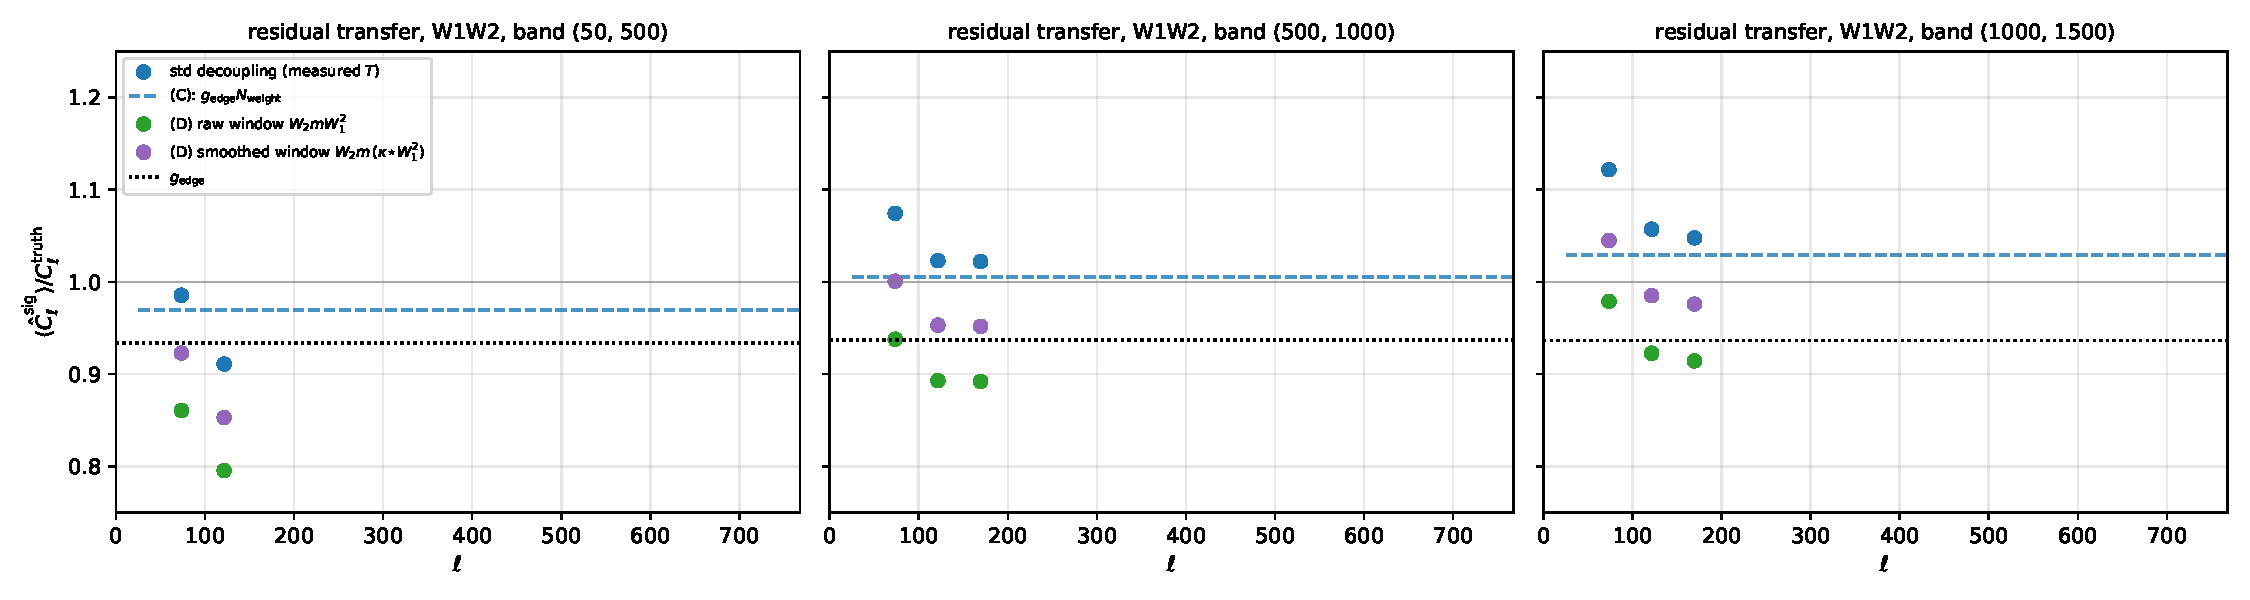
\includegraphics[width=\textwidth]{figures/transfer_D_ns1024.pdf}
\caption{Residual transfer of the \textbf{W1W2} scheme under the standard
decoupling (blue points: measured; blue dashed: the closed form
$g_{\rm edge}N_{\rm weight}$ of \cref{eq:TC}) and under the method-(D) matrix
decoupling, with the raw window $\Wtwo{\rm m}\Wone^2$ (green) and the
kernel-smoothed window $\Wtwo{\rm m}(\kappa\star\Wone^2)$ of
\cref{eq:wDsmooth} (purple), for the $M_0$ channel per filter band, on the
signal-bearing bandpowers. The dotted line is $g_{\rm edge}$, the solid grey
line unity. The raw window over-corrects (lands below $g_{\rm edge}$); the
kernel-smoothed window absorbs both the $\Wone$ lift and the edge loss,
leaving a residual close to unity in the narrow bands.}
\label{fig:transferD}
\end{figure}

\paragraph{Spin-4.}
A scalar power modulation does not source $M_{4E}=\mathrm{Re}\,\xi^2$ at linear
order ($\E[\xi^2]=0$); its signal is the anisotropic (tidal) response, with a
different kernel and amplitude. The \emph{geometric} transfer
\cref{eq:TC} --- mask$\,\otimes\,$filter non-commutation and weight normalization
--- is, however, common to both spin channels, as confirmed by the near-equal
measured $M_0$ and $M_{4E}$ transfers (\cref{tab:chi2}). We therefore compare the
scalar prediction with both measured channels in \cref{fig:transfer_pred}.

\begin{figure}[t]
\centering
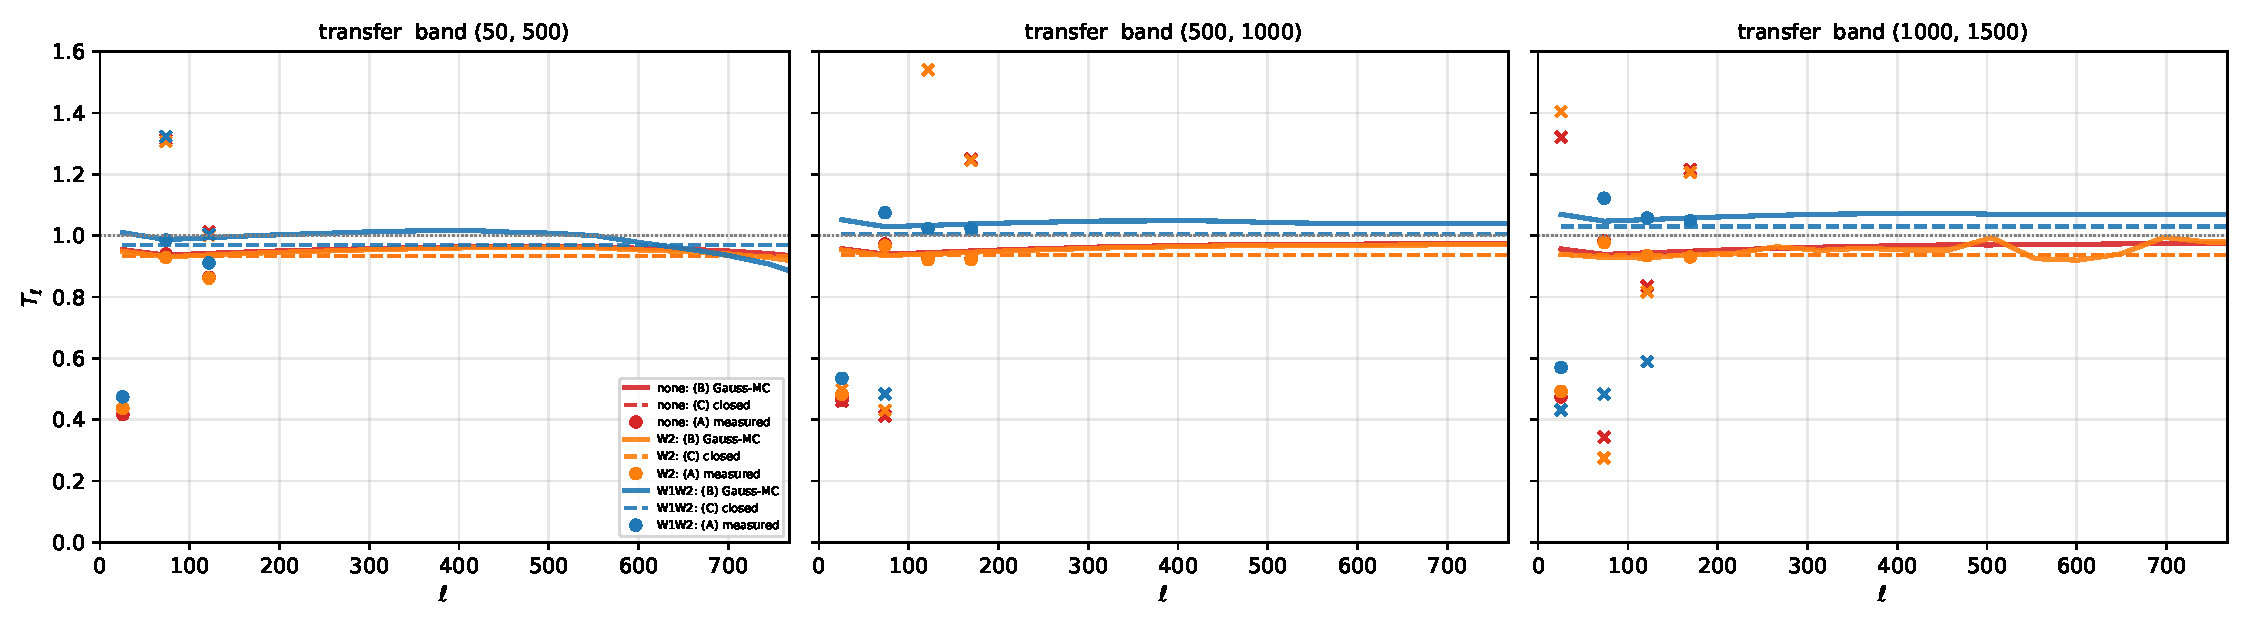
\includegraphics[width=\textwidth]{figures/transfer_pred_ns1024.pdf}
\caption{Transfer function by the three methods over the full analysed range
$\ell\le768$, per scheme (colour) and band. Points: measured (A) for $M_0$
(circles, signal-bearing bandpowers) and $M_{4E}$ (crosses). Solid lines:
Gaussian Monte-Carlo (B); dashed: closed form (C), \cref{eq:TC}. The predictions
use only the fixed $\delta_{\rm src}$ survey window (hence $\Wone,\Wtwo$), the
spectra $C^{\gamma\gamma}$ (via $\kappa$) and $C^{\dt\dt}$, the mask and the
filter --- and never the lens map. (B) and (C) agree, and both match the
measured transfer to $\sim$1--3\% in the narrow bands $[500,1000]$ and
$[1000,1500]$ --- including the \textbf{W1W2} lift to $\simeq1.0$--$1.05$ --- and
to $\sim$8\% in the wide low band $[50,500]$, where the white-band approximation
for $\kappa$ is least accurate (cf.\ the optimal-weights note). The lift is thus a
deterministic inverse-variance effect, not a source--lens correlation; both spin
channels follow the common scalar prediction. (The lowest bandpower of the measured $T$ is noisy:
the mode-coupling matrix is ill-conditioned for the largest scales on an
$\sim\!11\%$ footprint.)}
\label{fig:transfer_pred}
\end{figure}

\end{document}
